\documentclass[cmfonts]{witpress}
\usepackage{todonotes}
\usepackage{siunitx}
\usepackage{amsmath}
\usepackage{bm}
\usepackage{cleveref}
\usepackage{amssymb}
\usepackage{subcaption}
\captionsetup{compatibility=false}
% \usepackage{natbib}
\bibliographystyle{witpress}


\begin{document}


\title{Improvement of crash forces in structures using optimization tools.}

\author{L. E. Romera, L. Pire, M. Costas, J. Paz, J. D\'iaz, S. Hern\'andez.}

\address{Structural Mechanics Group, Universidade da Coru\~na, Spain.}

\maketitle

\begin{abstract}
This work describes an investigation on the structural optimization of the crash response of aircraft or road vehicle crash boxes, where the force pulse due to frontal impact or hard landing wanted to be kept as stable as possible while reducing the mass of the energy absorbing systems. The objective functions were minimized in a multi-objective approach using metamodeling on FE models and genetic evolutionary algorithms. Finite element models were subjected to a frontal impact test against a simplified rigid wall in the case of the car model, or to hardlanding impact for the fuselage model. Force-time curves was obtained from the analysis and suitably filtered. The objective functions were calculated as the variance of this force-time curves and the total structural mass. The objective was to obtain a force-time curve which was as close as possible to the ideal dissipator curve, with lower values of the peaks of acceleration experienced by the occupants; and to minimize the mass for fuel saving and environmental reasons. To that end, optimization strategies were planned carefully to deal with problems which are typical in crashworthiness optimization like expensive computation times and numerical noise.
\end{abstract}\\
\emph{Keywords: crashworthiness, injuries reduction, size optimization, surrogate models.}

\section{Introduction}
Occupant safety is a key issue on vehicle and aircraft design nowadays, and crashworthy elements are required to absorb the energy during a crash and minimize the effects on the occupants. Aircraft and vehicles are nowadays provided with crash boxes to absorb the impact energy through deformation in order to protect the passengers. They are usually tube-shaped and made of several parts that require some kind of bonding.

On the other hand, structural adhesives have improved their mechanical properties in recent years and can be now used with confidence in heavy duty applications. Interest on them is also raising up in scientific fields thanks to these enhancements and to the recent development of validated numerical models.
\begin{figure}[htpb]
	\centering
	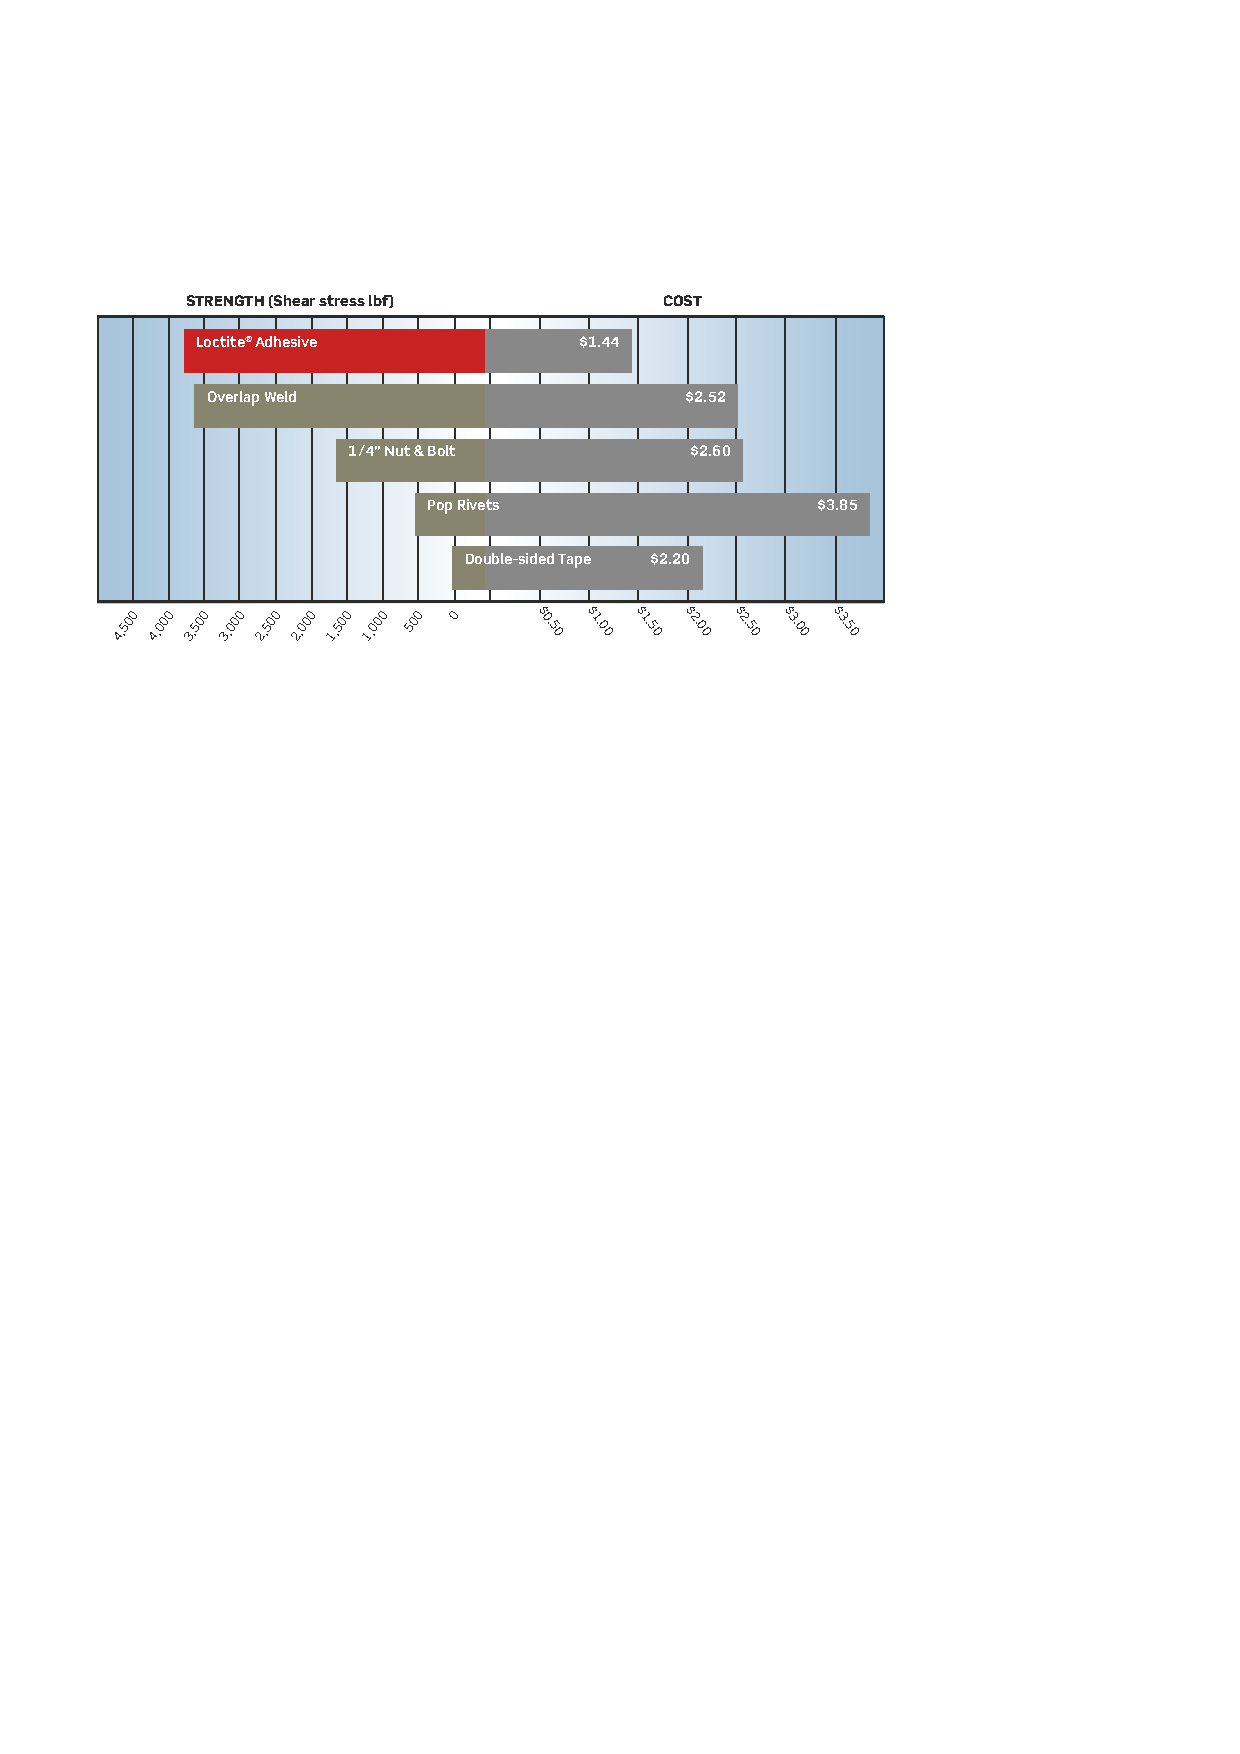
\includegraphics[width=\linewidth]{./figures/IMG_CUTRES/comparison}
	\caption[Qualitative strength and cost comparison of different joining solutions.]{Qualitative strength and cost comparison of different joining solutions. Taken from \cite{superyacht}.}
	\label{fig:comparison}
\end{figure}

As shown in \Cref{fig:comparison}, adhesives are very competitive both in bonding strength and in economical manufacturing costs \cite{superyacht}. In order to check adhesive's suitability for their use in crashworthy elements, this research develops numerical models of adhesively bonded crash boxes subjected to impact loads using finite element models. Information and data present in the literature are used to create and validate these models in order to ensure the accuracy of the results.

\section{Finite element model}
The modeled crash box consists of two adherend cold-formed sheets made of steel that create a tube of square section bonded together with an epoxy adhesive. The joint is practiced on the surface of two flanges on each adherend side. In order to ease the model validation, the crash box geometry was created to reflect those tested by \cite{Peroni2009} and later modeled by \cite{Scattina2011}. In particular, the two sections depicted in \cref{fig:crash_box} are modeled in the present study.

\begin{figure}[ht]
  \centering
  \begin{minipage}[b]{.48\linewidth}
    \centering
    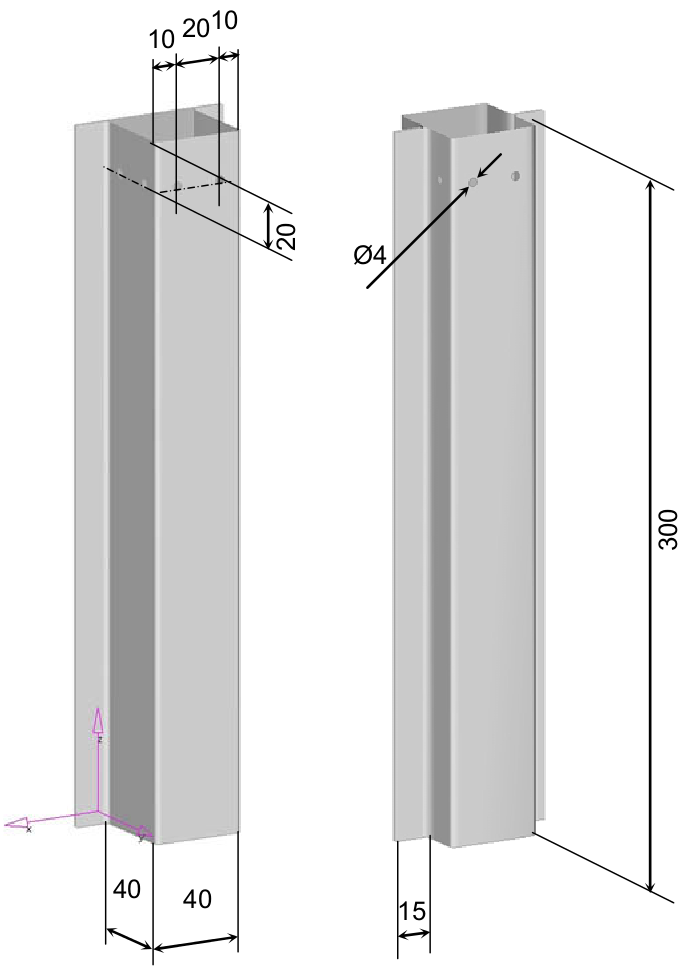
\includegraphics[width=\linewidth]{figures/IMG_CUTRES/medidas_cb}
    \subcaption{Dimensions of the modeled crash boxes, in millimeters. Taken from \cite{Peroni2009}.}
    \label{fig:crash_box}
  \end{minipage}
  \hfill
  \begin{minipage}[b]{.48\linewidth}
    \centering
    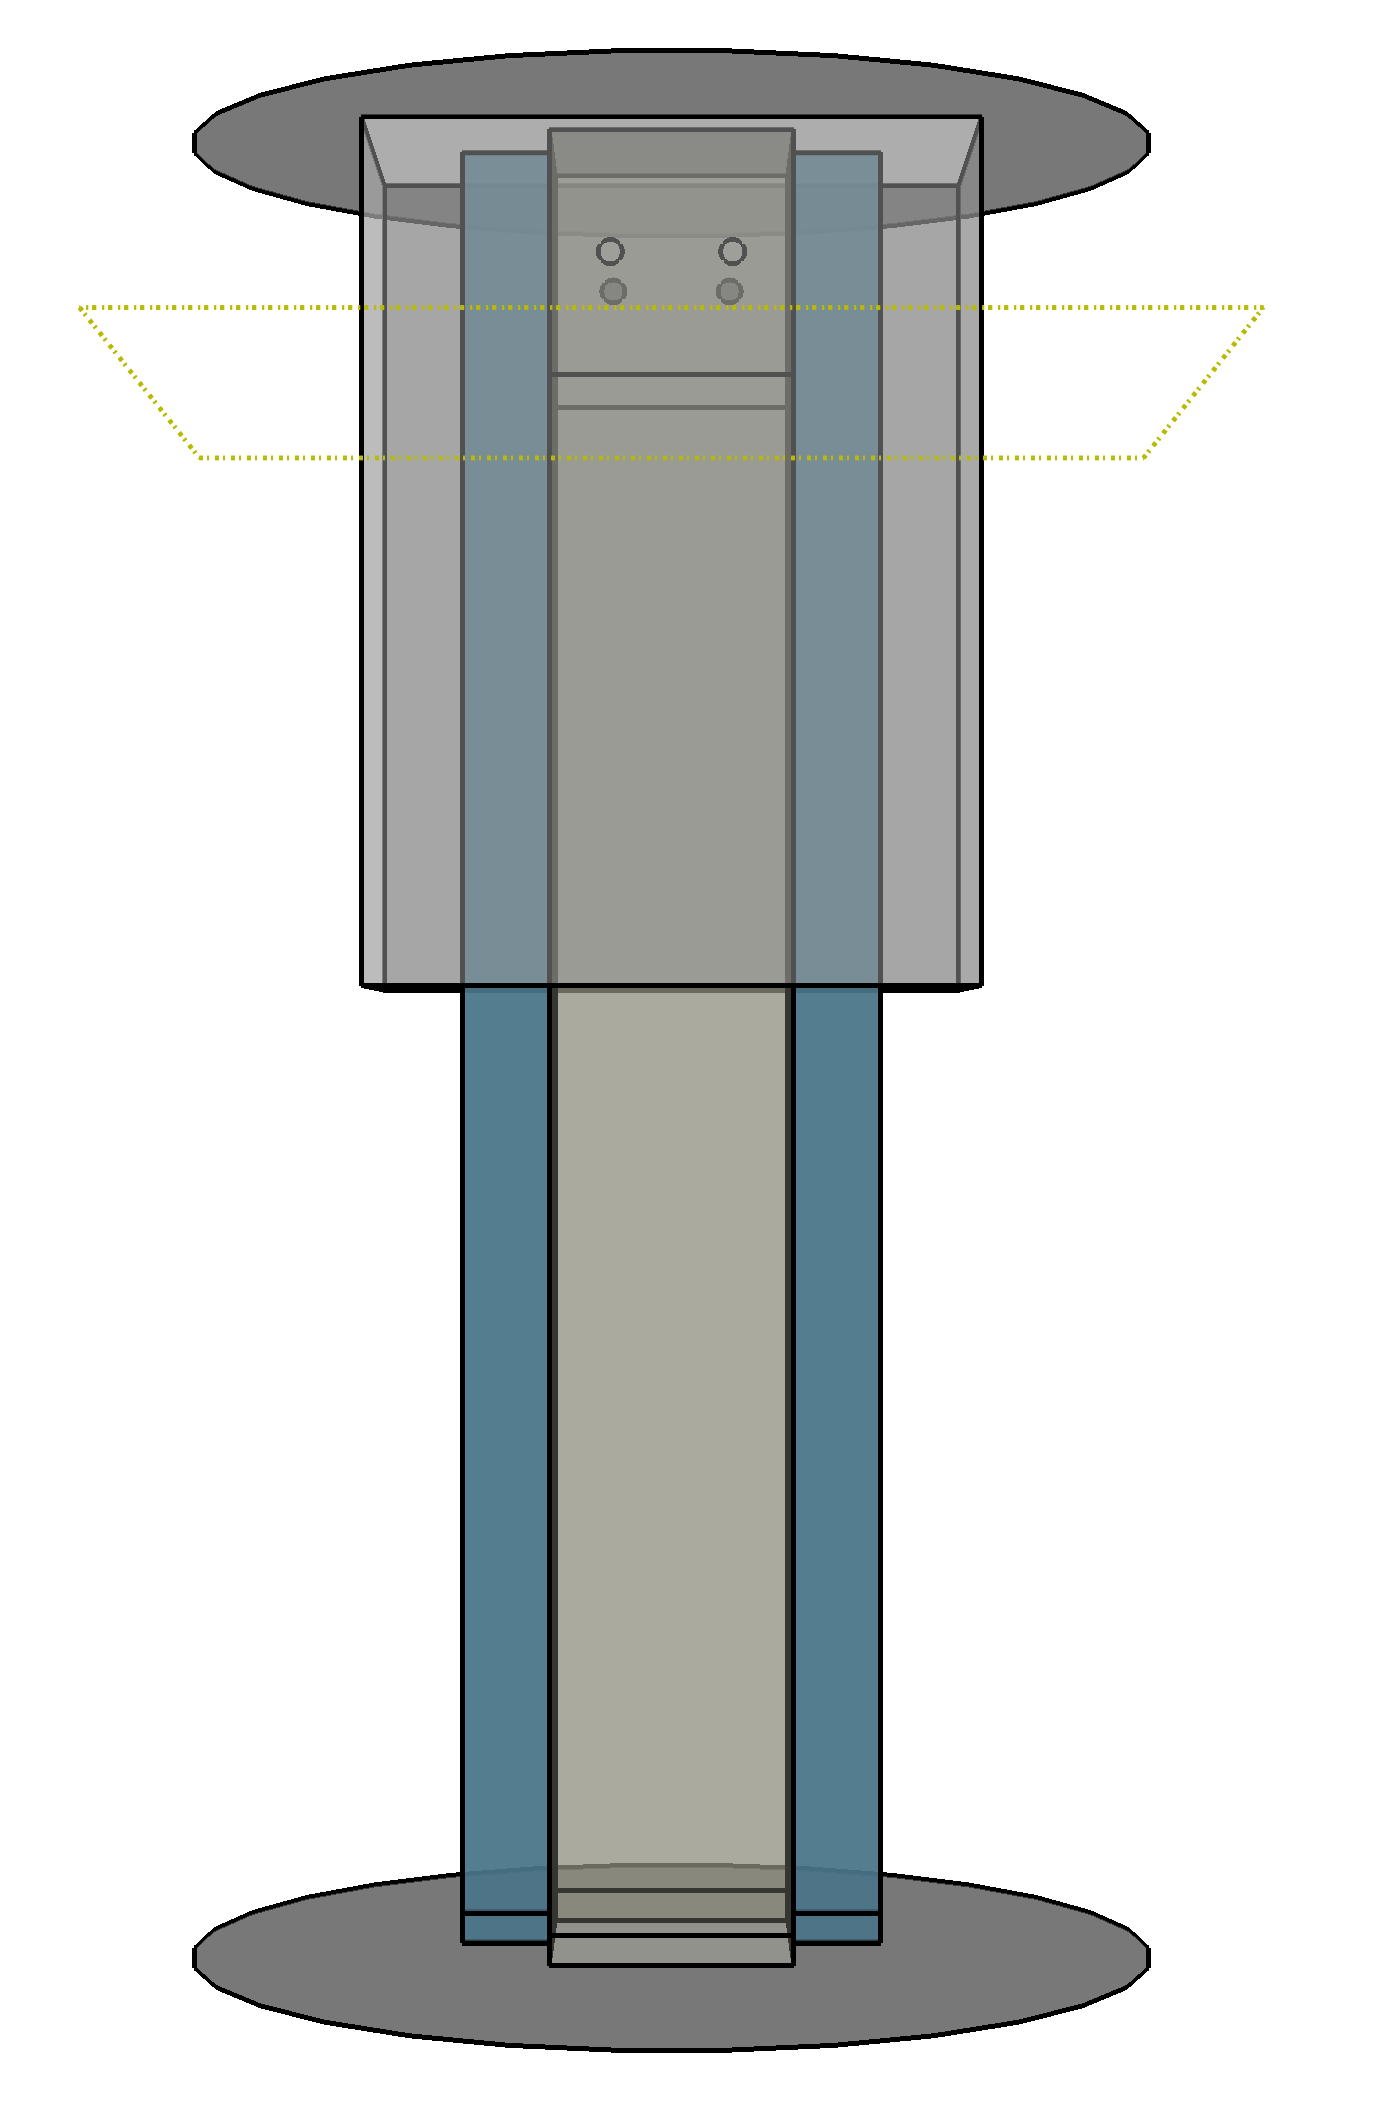
\includegraphics[width=0.9\linewidth]{figures/IMG_CUTRES/general_transp}
    \subcaption{General view of the model with the bounding box.}
    \label{fig:general}
  \end{minipage}
  \caption{Dimensions of the studied crash boxes and view of the finite element model including a bounding box.}
  \label{fig:modelo}
\end{figure}

\todo{centrar figuras}

The tube is crushed between two rigid plates, one fixed and the other moving at impact speed (see \Cref{fig:general}). In order to ease the formation of a stable collapse mechanism, a triggering is machined near the front end of the tube. The trigger starts a desired collapse mode in that area. Due to the high slenderness of the tube, difficulties were found in order to achieve stable collapse mechanisms. On their place, tubes diverted from their axis. Trying to avoid these critical situations, four rigid plates on a rectangular section around the crash tube were added to the model as a bounding box. Its section was $\num{100}\times\SI{60}{\mm}$ and co-centered with the crash box.

The impact plate moved during the simulation at $\SI{10}{\m/\s}$ on a total distance equal to half of the total tube's length, resulting in a total analysis time of $\SI{0.015}{\s}$. Rotational degrees of freedom were fixed on the frontal plate. The rear plate had all degrees of freedom restrained.

The last $\SI{5}{\mm}$ of the crash tube had all degrees of freedom fixed (see \cref{fig:general}), except displacement on the impact direction in order to allow the reaction force measurement commented before. This way, numerical issues due to excesive unrestrained degrees of freedom on the whole tube were prevented.

Peeling problems were found near the impact head end during the development of the study. \cite{Peroni2009} solved this situation by adding two rivets on the bonded flanges at the triggered section in order to avoid excesive debonding on that part of the tube in the initial phases of the impact and, thus, prevent critical situations. In this study, this was simulated by a $\SI{2}{\mm}$-diameter spot-weld at the same location.

\subsection{Materials}

The model is made up of two different materials: the adherends of the tube are made of steel and the adhesive is the epoxy-based, heat-cured Loctite Hysol 9514.

According to \cite{manufCatalog}, the shear strength of the adhesive is $\SI{44}{\MPa}$, although this parameter is subject to variation depending both in cure temperature and time. The bulk modulus is $\SI{1460}{\MPa}$ and the adhesive's density is $\SI{1.30}{\tonne/\m^3}$ \cite{manufCatalog}. The constitutive behavior was supposed to be isotropic linear elastic \cite{SernaMoreno2015} up to failure start. An uncoupled traction elastic behavior \cite{Sadowski2010, Sadowski2011, Scattina2011, Sadowski2014} on 3D cohesive finite elements was chosen.

\cite{Scattina2011} obtained adhesive stiffnesses through the inverse method, which are summarized in \cref{tab:ads_params}. These same parameters were used in the present study, as their results could be validated with the model.

\begin{table}
	\centering
	\begin{tabular}{llrl}
	\hline
		Parameter & Description & Value & \\
		\hline
		$E_{N}$ & Stiffness in normal direction & $\num{5e9}$ & $\si{\kN/\m^2}$ \\
		$E_{T}$ & Stiffness in an in-plane direction & $\num{8e7}$ & $\si{\kN/\m^2}$ \\
		$G_{Ic}$ & Energy release rate for mode I & $\num{2028}$ & $\si{\J/\m^2}$ \\
		$G_{IIc}$ & Energy release rate for mode II & $\num{11853}$ & $\si{\J/\m^2}$ \\
		$\sigma_{n}^{0}$ & Peak traction in normal direction & $\num{130}$ & $\si{\MPa}$ \\
		$\tau_{II}^{0}$ & Peak traction in tangential direction & $\num{42.5}$ & $\si{\MPa}$ \\
		\hline
	\end{tabular}
	\caption[Loctite Hysol 9514 parameters.]{Loctite Hysol 9514 parameters. Taken from \cite{Scattina2011}.}
	\label{tab:ads_params}
\end{table}

Contact failure modeling ---corresponding to adhesive failure--- resulted in some simulation problems, so adhesives and adherends were kept together with a simplified tie constraint. Thus, failure definitions were only included in the bulk material, obviating the contact/adhesive failure as suggested by several authors \cite{Greve2007, Loureiro2010, Sadowski2010, Sadowski2011, Scattina2011, Sadowski2014, SernaMoreno2015}, although the modeled cohesive damage parameters include the effect of both adhesive and cohesive resistance. The quadratic nominal stress criterion is a damage initiation criterion, defined as
\begin{equation}
\left(\frac{\left<\sigma_{n}\right>}{\sigma_{n}^{0}}\right)^{2} + \left(\frac{\tau_{II}}{\tau_{II}^{0}}\right)^{2} + \left(\frac{\tau_{III}}{\tau_{III}^{0}}\right)^{2} = 1 ;
\label{eq:quads}
\end{equation}
where $\sigma_{n}^{0}$, $\tau_{II}^{0}$ and $\tau_{III}^{0}$ represent the pure mode loading threshold stresses for each direction. The out-of-plane value, $\sigma_{n}^{0}$, was set to $\SI{42.5}{\MPa}$ \cite{Scattina2011}, which corresponds to the peeling failure stress for steel. Note that Macaulay brackets indicate that compression is not considered in failure initiation. Both in-plane values, $\tau_{II}^{0}$ and $\tau_{III}^{0}$, were set to $\SI{130}{\MPa}$ \cite{Scattina2011}. These values are also included in \cref{tab:ads_params}. % ref to catalog?

As long as the condition exposed in \cref{eq:quads} is not satisfied, the adhesive layer behaves elastically. Once the condition gets satisfied, damage starts and a degradation in stiffness can be appreciated following the specified damage evolution model. For this particular case, the material degradation was set as a fracture energy power law, as given by \cref{eq:fracture_energy}.

\begin{equation}
\left(\frac{G_{I}}{G_{Ic}}\right)^{\alpha}+\left(\frac{G_{II}}{G_{IIc}}\right)^{\alpha}+\left(\frac{G_{III}}{G_{IIIc}}\right)^{\alpha}=1 ;
\label{eq:fracture_energy}
\end{equation}
where $G_{Ic}$ corresponds to the critical fracture energy required to cause failure in mode I (out-of-plane direction), and being $G_{IIc}$ and $G_{IIIc}$ the values for mode II and III, respectively, which correspond to both shear directions. The critical fracture energy for the Loctite Hysol 9514 in the normal direction is $\SI{2028}{\J/\m^2}$ \cite{Scattina2011}. It was considered that the adhesive had no preferential directions for tangential failure, meaning $G_{IIc}$ was equal to $G_{IIIC}$, and being the fracture energy equal to $\SI{11853}{\J/\m^2}$ \cite{Scattina2011}. These values are also provided in \cref{tab:ads_params}. The exponent $\alpha$ was considered equal to $\num{2}$ \cite{Loureiro2010, Sadowski2010, SernaMoreno2015}.

Regarding the metal sheets, in order to make the model comparable to the experiments carried out by \cite{Peroni2009}, steel was chosen for these adherends. In the present study, it is defined as an isotropic elastic-plastic material, with a density of $\SI{7.85}{\tonne/\m^3}$.

The elastic part of the adherend stress-strain curve is defined as linear, with an elastic modulus of $\SI{200}{\GPa}$ and a Poisson ratio of $\num{0.3}$. An initial yield stress of $\SI{190}{\MPa}$ is set, and work hardening is defined through a tangent plastic modulus of $\SI{950}{\MPa}$ \cite{Peroni2009}.



\subsection{Finite element mesh and simulation setup}

The use of cohesive elements allowed to make the adhesive's mesh much coarser due to their aspect ratios requirements. These elements were created with a size of $\SI{2.0}{\mm}$, and had only one element in the $\SI{0.3}{\mm}$ layer thickness. Other tested element types, specifically solids, had problems if side lengths were bigger than about $\SI{0.5}{\mm}$, and were completely unfeasible with lengths larger than $\SI{1.0}{\mm}$ approximately.

% Tie (include image)
The tie constraint included in Abaqus enabled non-coherent meshes between adhesive and adherend (\cref{fig:mesh_detail_coh3d_comparison}). This way, finer meshes could be implemented on the adhesive in order to improve the representation of the failure progression without increasing the adherend element recount by leaving a coarser mesh there.

\begin{figure}[htpb]
	\centering
	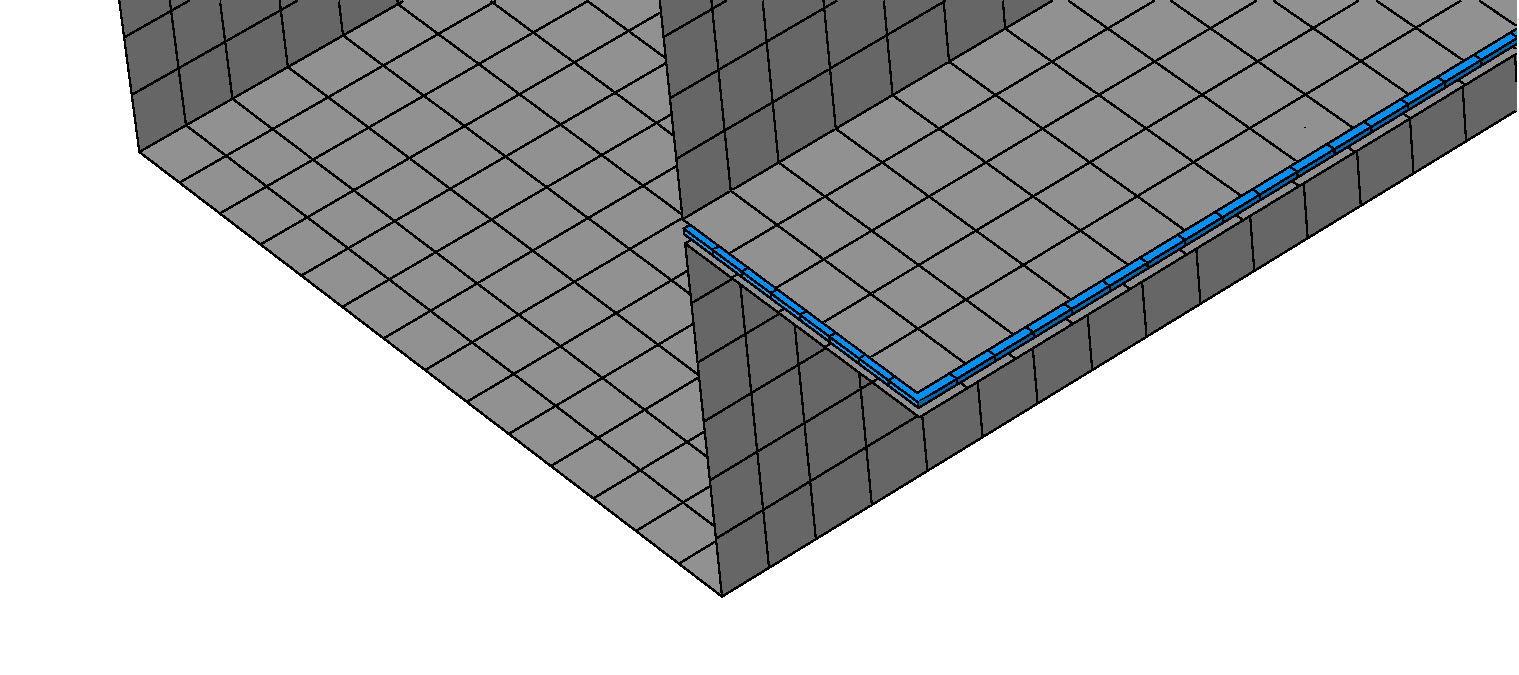
\includegraphics[width=0.7\linewidth]{figures/IMG_CUTRES/mesh_detail_coh3d_comparison}
	\caption[Detail of COH3D mesh on the adhesive layer.]{Detail of COH3D mesh on the adhesive layer (blue).}
	\label{fig:mesh_detail_coh3d_comparison}
\end{figure}

\Cref{fig:mesh} shows the used mesh for the crash tube, which has more than $\num{10600}$ elements.
\begin{figure}[htpb]
	\centering
	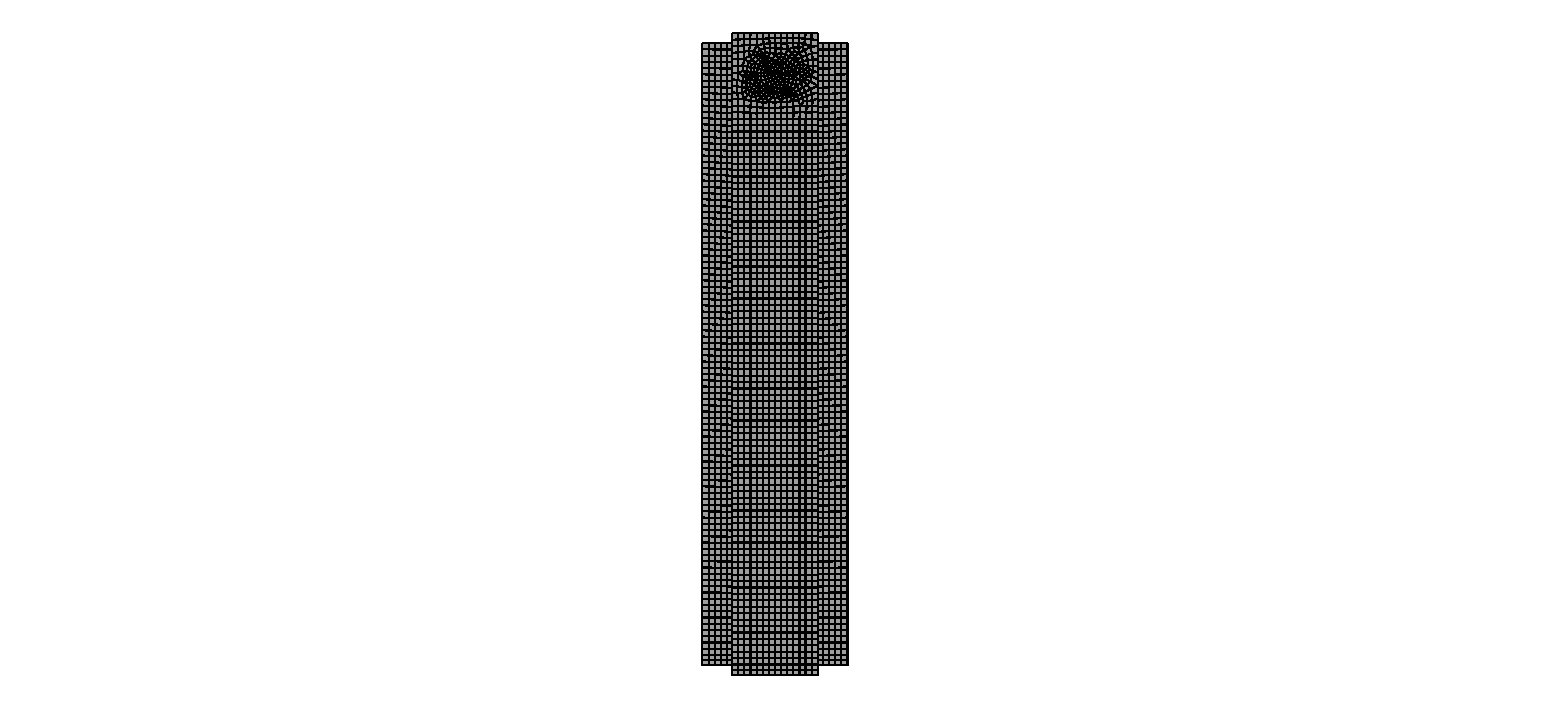
\includegraphics[width=0.9\linewidth]{figures/IMG_CUTRES/mesh}
	\caption{General mesh of the crash box.}
	\label{fig:mesh}
\end{figure}

The finite element package Abaqus Explicit is used in this research, on is version 6.13 \cite{Abaqus613Manual} running on a high performance computing cluster. Jobs running on loop parallelization over $16$ cores took about $\SI{8}{\hour}$ to finish. Domain parallelization turned out to be inefficient in this case due to poor network performance.

\subsection{Simulation results}


In order to filter high frequency effects, a SAE 600 filter was applied to the simulation results \cite{Huang}. \Cref{fig:F-D_frictionless,fig:F-D_rough} provide the force-displacement curves considering no friction and rough interaction properties respectively. In that same figure and in the upcoming ones, nomenclature is as follows:
\begin{itemize}
	\item ``A'' or ``B'' indicating the cross-section of the tube: ``A'' for the top-hat, and ``B'' for the double hat.

	\item Following that, ``R'', indicating that the rough tangential contact property was used, or ``Fl'', for the frictionless case.

	\item An ``R'' after the underline indicates that the crash box had riveting in the triggered cross section.

	\item ``Sb'' after the underline marks the presence of a stabilizing box in the model.
\end{itemize}

\begin{figure}
	\centering
	\begin{minipage}[b]{.9\linewidth}
		\centering
		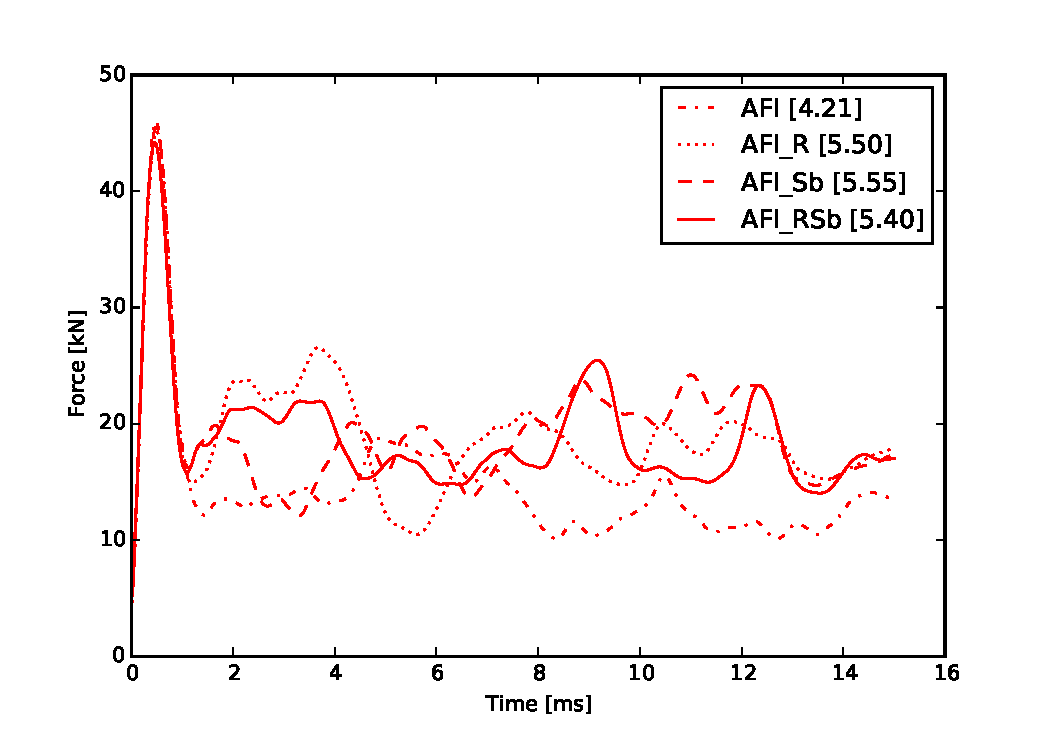
\includegraphics[width=\linewidth]{IMG_CUTRES/AFl}
	\end{minipage}
	\quad
	\begin{minipage}[b]{.9\linewidth}
		\centering
		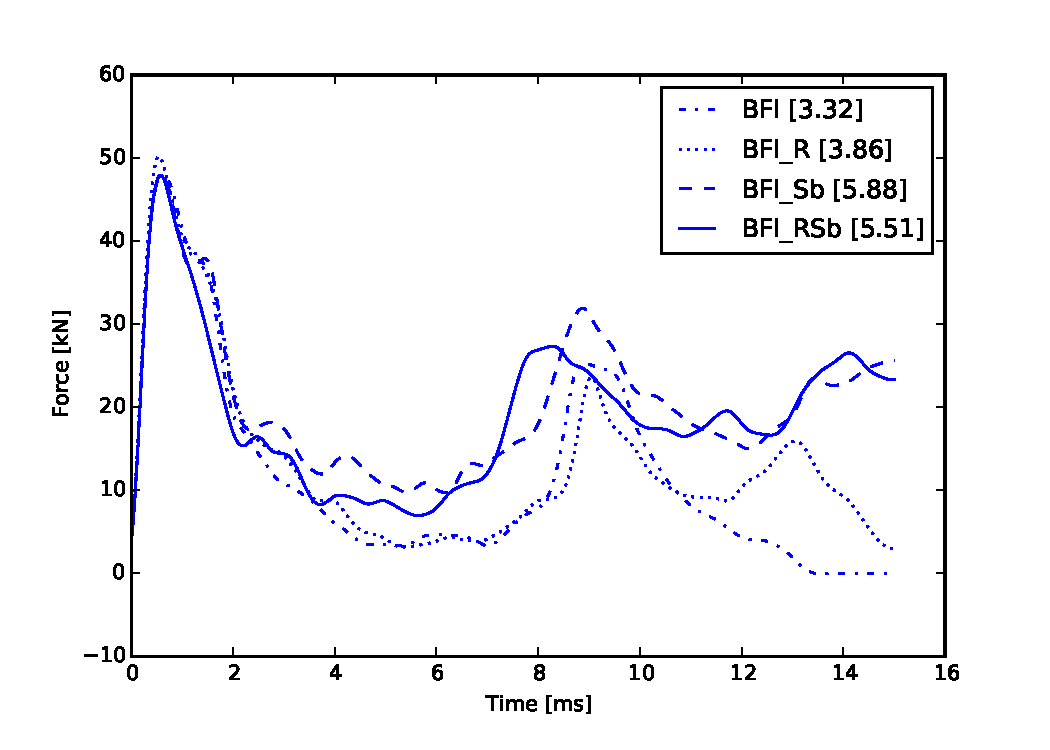
\includegraphics[width=\linewidth]{IMG_CUTRES/BFl}
	\end{minipage}
	\caption[F-D for modeled cross sections, both top-hat and double hat, with different modeled configurations with frictionless contact.]{F-D for modeled cross sections, both top-hat (red) and double hat (blue), with different modeled configurations with frictionless contact. SEA values in brackets in $\si{\kJ/\kg}$.}
	\label{fig:F-D_frictionless}
\end{figure}

\begin{figure}
	\centering
	\begin{minipage}[b]{.9\linewidth}
		\centering
		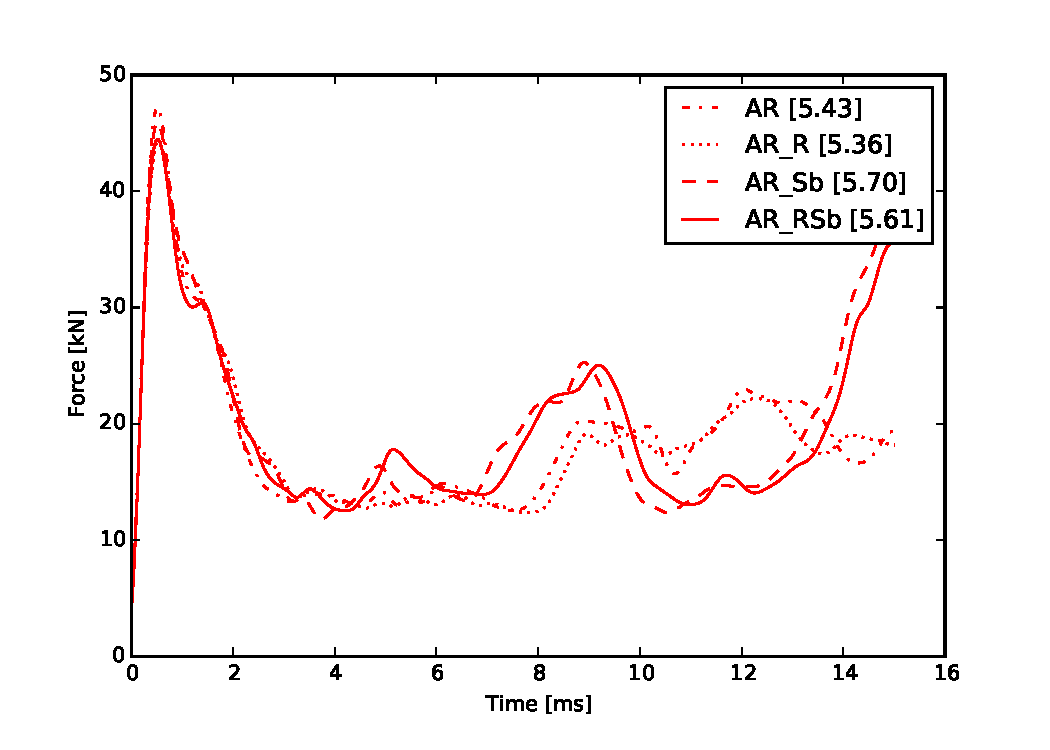
\includegraphics[width=\linewidth]{IMG_CUTRES/AR}
	\end{minipage}
	\quad
	\begin{minipage}[b]{.9\linewidth}
		\centering
		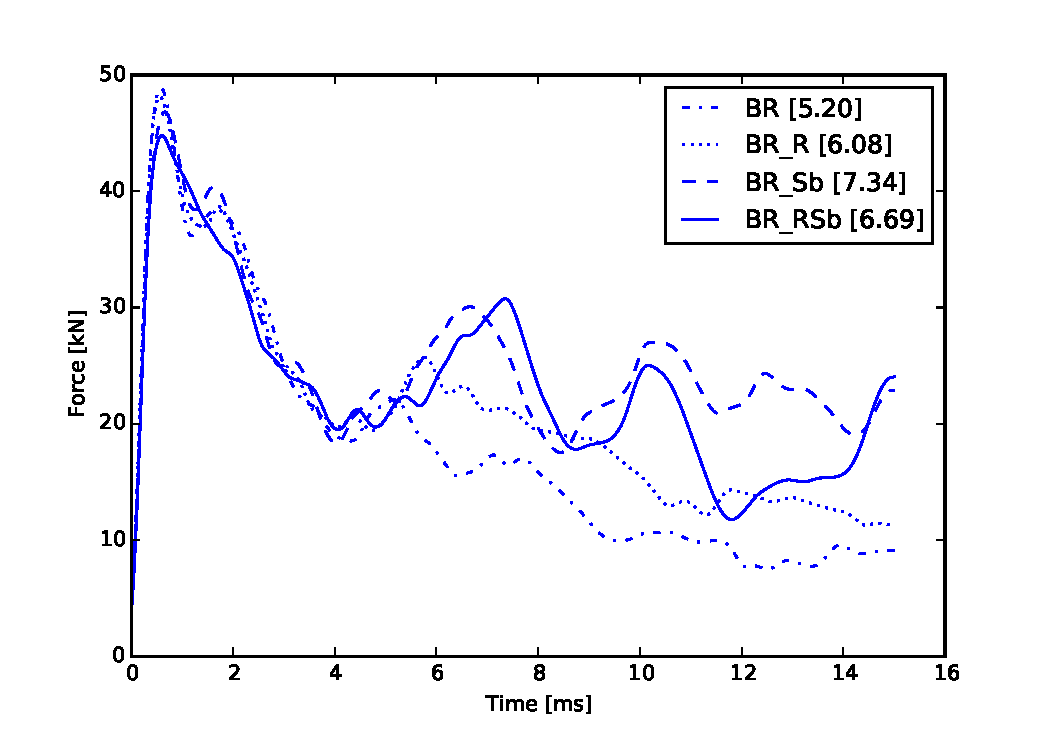
\includegraphics[width=\linewidth]{IMG_CUTRES/BR}
	\end{minipage}
	\caption[F-D for modeled cross sections, both top-hat and double hat, with different modeled configurations with rough contact.]{F-D for modeled cross sections, both top-hat (red) and double hat (blue), with different modeled configurations with rough contact. SEA values in brackets in $\si{\kJ/\kg}$.}
	\label{fig:F-D_rough}
\end{figure}

\begin{figure}
	\centering
	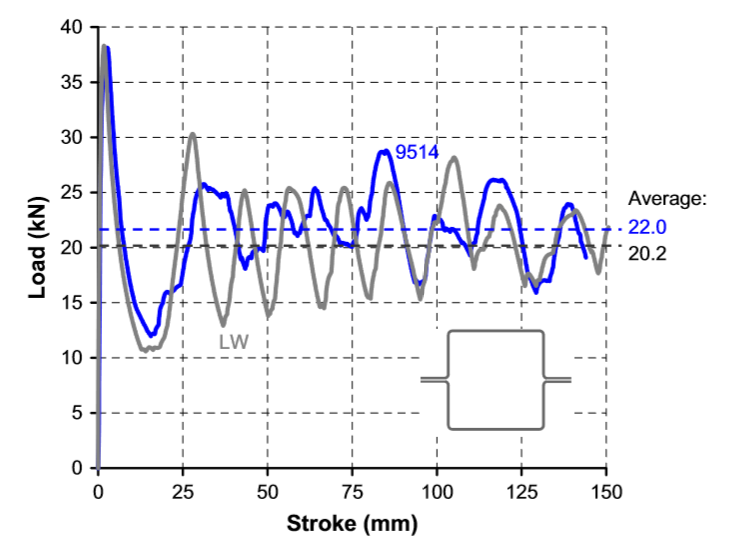
\includegraphics[width=0.7\linewidth]{IMG_CUTRES/peroni_qstat_fd}
	\caption[F-D obtained by \cite{Peroni2009} in quasi-static test for studied adhesive and other bonding solution.]{F-D obtained by \cite{Peroni2009} in quasi-static test for studied adhesive (blue) and other bonding solution (gray).}
	\label{fig:peroni_qstat_fd}
\end{figure}

Qualitatively, this curves are very similar to those obtained by \cite{Peroni2009}. \Cref{fig:peroni_qstat_fd} depicts a quasi-static test performed by these authors with the same section and bonding solution. Facing these similitudes, the model is considered valid.

In general, a uniform force-displacement curve would be the most desirable scenario, as it would imply maximizing the $E_\text{a}$  with the minimum $P_\text{peak}$. Thus, the best solution will be the one with the most constant-like behavior.

\subsubsection{Mean and standard deviation}

The mean and the SD of F-D are measured in each case. The former one is the least interesting of both, as it is directly related to SEA, which is already being calculated.

However, SD is fair more interesting for the analysis, as it gives an idea of the uniformity of the F-D during the analysis time span. As high values of the transmitted force are origin of injury of the occupants, the most uniform resulting curve will be the one with the lesser values of local peaks for the same mean load, and thus, the more desirable.

\section{Collapse mechanism}

The origin of the mentioned difference between quasi-static and impact results may be related to the collapse mechanism. Specifically, to the rate of changing the response mechanism for the crash box, from in-plane compression of the plates ---which is directly related to Pk---, to the initiation of wave formation. In the developed model, if compared to the collapse images provided by \cite{Scattina2011}, this rate is far slower. The last local peak of the F-D does not take place within the simulation interval due to a longer time span of the main peak.

\subsection{Wave formation}
\label{sec:wave_formation}

Crash box plates bending is the main way of energy absorption through elastic-plastic deformation. Wave formation consists on the formation of a series of foldings along the plates of alternating directionality, so the geometric axis of the tube is approximately kept in place, as it can be seen on \cref{fig:waves}. The non-accomplishment of this last condition is a case of critical situation.

\begin{figure}
\centering
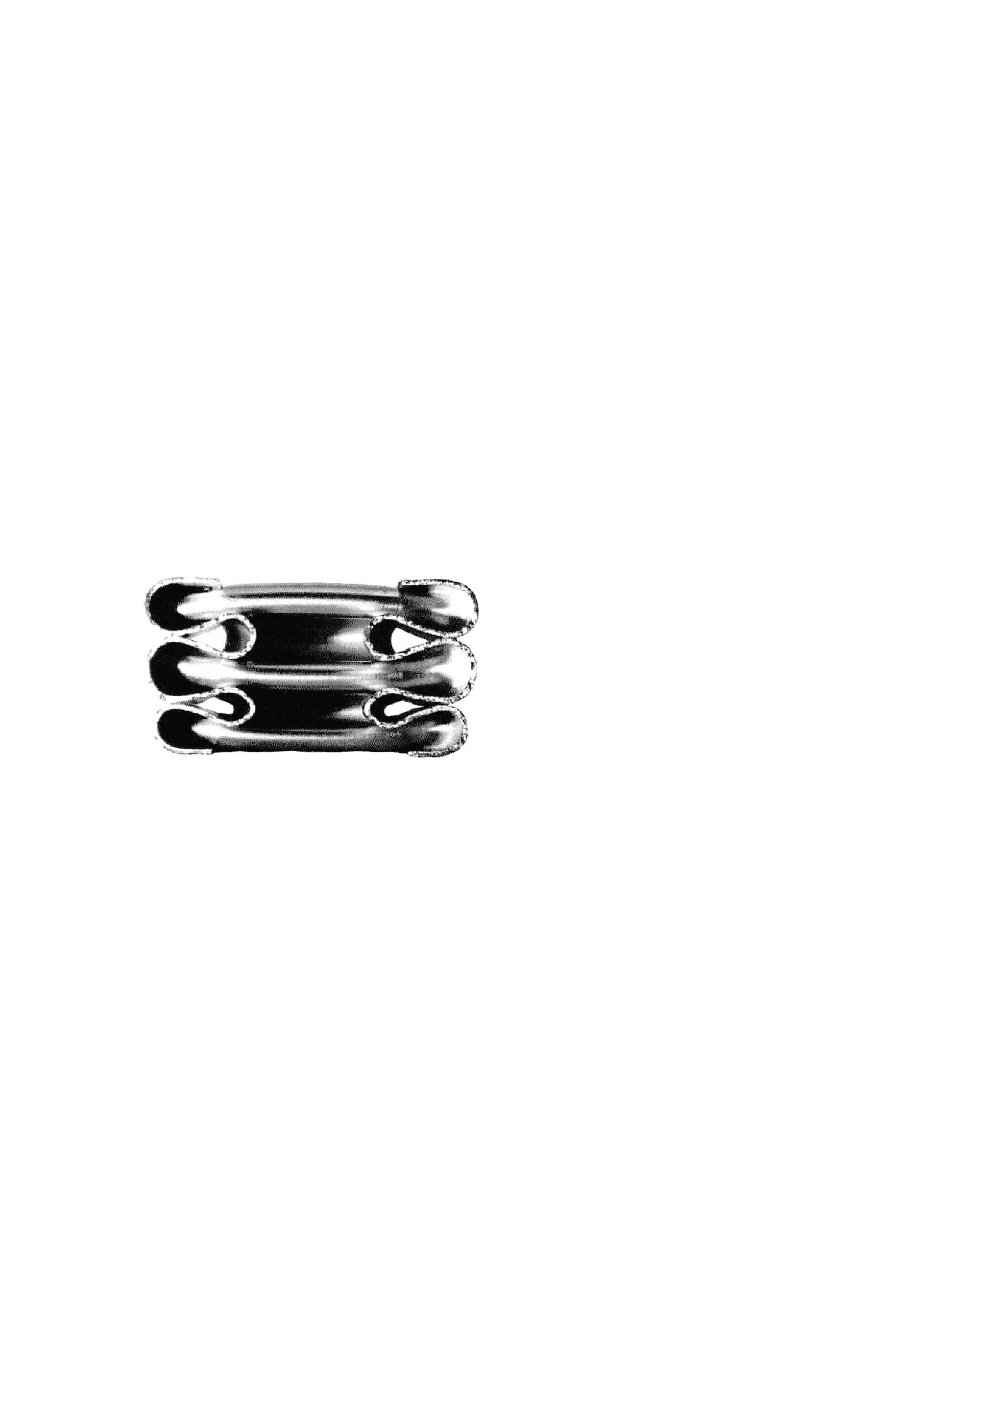
\includegraphics[width=0.7\linewidth]{figures/IMG_CUTRES/waves}
\caption[Waves formed on a crushed tube.]{Waves formed on a crushed tube. Taken from \cite{Langseth}.}
\label{fig:waves}
\end{figure}

It is in the wave formation process where another remarkable difference from the models tested by \cite{Scattina2011} takes place. In the present study, although waves develop sequentially as they were expected to, some simultaneity can be perceived on a certain length of the tube in some cases, like the one represented in \cref{fig:wave_form}. This is not considered binding of the validity of the model as, apart from happening on the impact head, wave formation may take also place in the opposite end of the tube or in some mid-point \cite{Abedrabbo2009, Costas2013} in this slender crash devices.

\begin{figure}
	\centering
%	\begin{minipage}[b]{.08\linewidth}
%		\centering
%		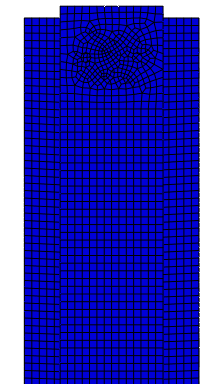
\includegraphics[width=\linewidth]{IMG_CUTRES/c0}
%	\end{minipage}
%	\quad
	\begin{minipage}[b]{.15\linewidth}
		\centering
		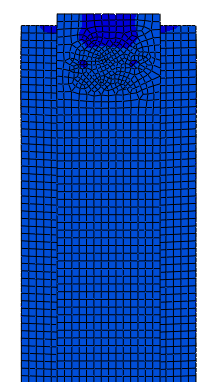
\includegraphics[width=\linewidth]{IMG_CUTRES/c1}
		$\SI{3}{\ms}$
	\end{minipage}
	\quad
	\begin{minipage}[b]{.15\linewidth}
		\centering
		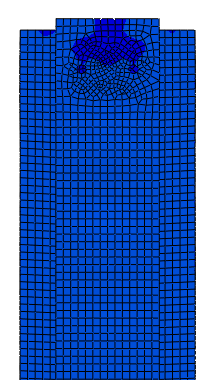
\includegraphics[width=\linewidth]{IMG_CUTRES/c2}
		$\SI{6}{\ms}$
	\end{minipage}
	\quad
	\begin{minipage}[b]{.15\linewidth}
		\centering
		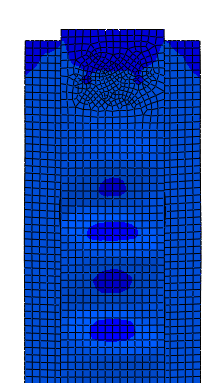
\includegraphics[width=\linewidth]{IMG_CUTRES/c3}
		$\SI{9}{\ms}$
	\end{minipage}
	\quad
	\begin{minipage}[b]{.15\linewidth}
		\centering
		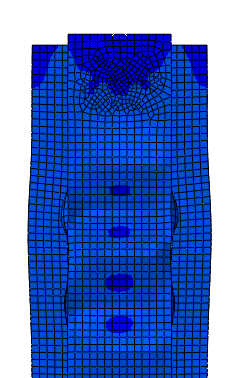
\includegraphics[width=\linewidth]{IMG_CUTRES/c4}
		$\SI{12}{\ms}$
	\end{minipage}
	\quad
	\begin{minipage}[b]{.15\linewidth}
		\centering
		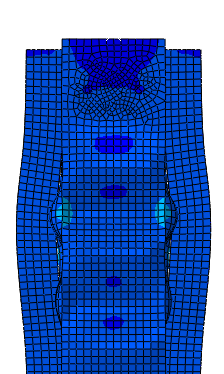
\includegraphics[width=\linewidth]{IMG_CUTRES/c5}
		$\SI{15}{\ms}$
	\end{minipage}
	\quad
	\begin{minipage}[b]{.15\linewidth}
		\centering
		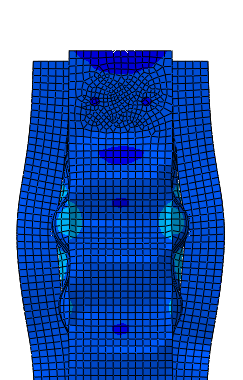
\includegraphics[width=\linewidth]{IMG_CUTRES/c6}
		$\SI{18}{\ms}$
	\end{minipage}
	\quad
	\begin{minipage}[b]{.15\linewidth}
		\centering
		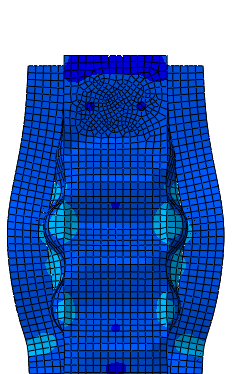
\includegraphics[width=\linewidth]{IMG_CUTRES/c7}
		$\SI{21}{\ms}$
	\end{minipage}
	\quad
	\begin{minipage}[b]{.15\linewidth}
		\centering
		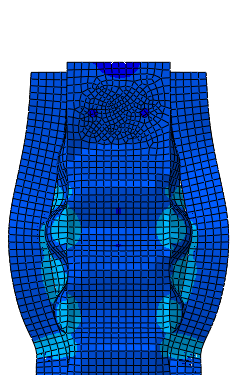
\includegraphics[width=\linewidth]{IMG_CUTRES/c8}
		$\SI{24}{\ms}$
	\end{minipage}
	\quad
	\begin{minipage}[b]{.15\linewidth}
		\centering
		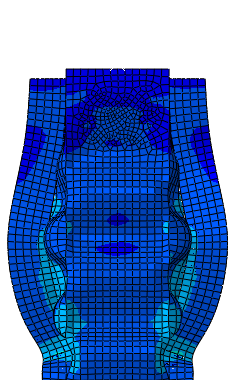
\includegraphics[width=\linewidth]{IMG_CUTRES/c9}
		$\SI{27}{\ms}$
	\end{minipage}
	\quad
	\begin{minipage}[b]{.15\linewidth}
		\centering
		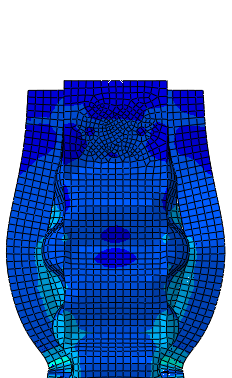
\includegraphics[width=\linewidth]{IMG_CUTRES/c10}
		$\SI{30}{\ms}$
	\end{minipage}
\caption{Early stages of wave formation process on the impact head.}
\label{fig:wave_form}
\end{figure}

During the development of this study, several adherend thicknesses were tried as a manner of influence on the simultaneity/sequentiality of the wave formation. It was checked that thicker adherends were proner to develop sequentiality in this process, although other problems arise, as it is explained later.

\subsection{Critical situations}
\label{sec:critical_sits}
\cite{Peroni2009} found several situations in impact tests in which the expected collapse mechanism wasn't achieved. Instead, bonding rapidly failed, making almost only use of the plate's capabilities to absorb the impact through its elastic-plastic deformation like bending shells, usually without wave formation at all or only on a part of the tube.

When this situation takes place, Ea may get drastically reduced, depending on several parameters. During the study development, it was found on several unprecise models ---i.e.: with minored adhesive properties--- that this critical situations can drop SEA to a half or even a third of the expected values if compared with non-critical values given by \cite{Peroni2009} on their stable counterparts. In some cases, the general effect of this has less importance, as it will be shown. As previously explained, crash boxes fairly improve their response to this situation by fixing togheter the adherends plates with rivets \cite{Peroni2009}.

Critical situations also take place on FEM models. \cite{Yang2012} found this happening on a double-hat hexagonal tube subjected to impact (\cref{fig:yangs_tube}) using a validated model with equivalent adhesive properties. \cite{Yamashita2013} also found this on impact tests and models of a top-hat tube, being the experimental and the modelled tests very similar in their results.

In this study, they were mainly found on double-hat square tubes, being the top-hat solution fairly more resistant to these problems.
% SELF EXAMPLE AND FIGURE

The importance of controlling this misfunctions also has to do with material efficiency, as the stable collapse mechanism reaches the greatest values of Ea, with a reasonable control of Pk.

In the present study, as previously stated, they were controlled by the addition of a stabilizing box and spot weld points in the flanges at the triggering cross section. Although they are not prevented completely, the general behavior of the tube is fairly improved, as it gets closer to what is expected when comparing to \cite{Peroni2009} and \cite{Scattina2011}.

\begin{figure}
	\centering
	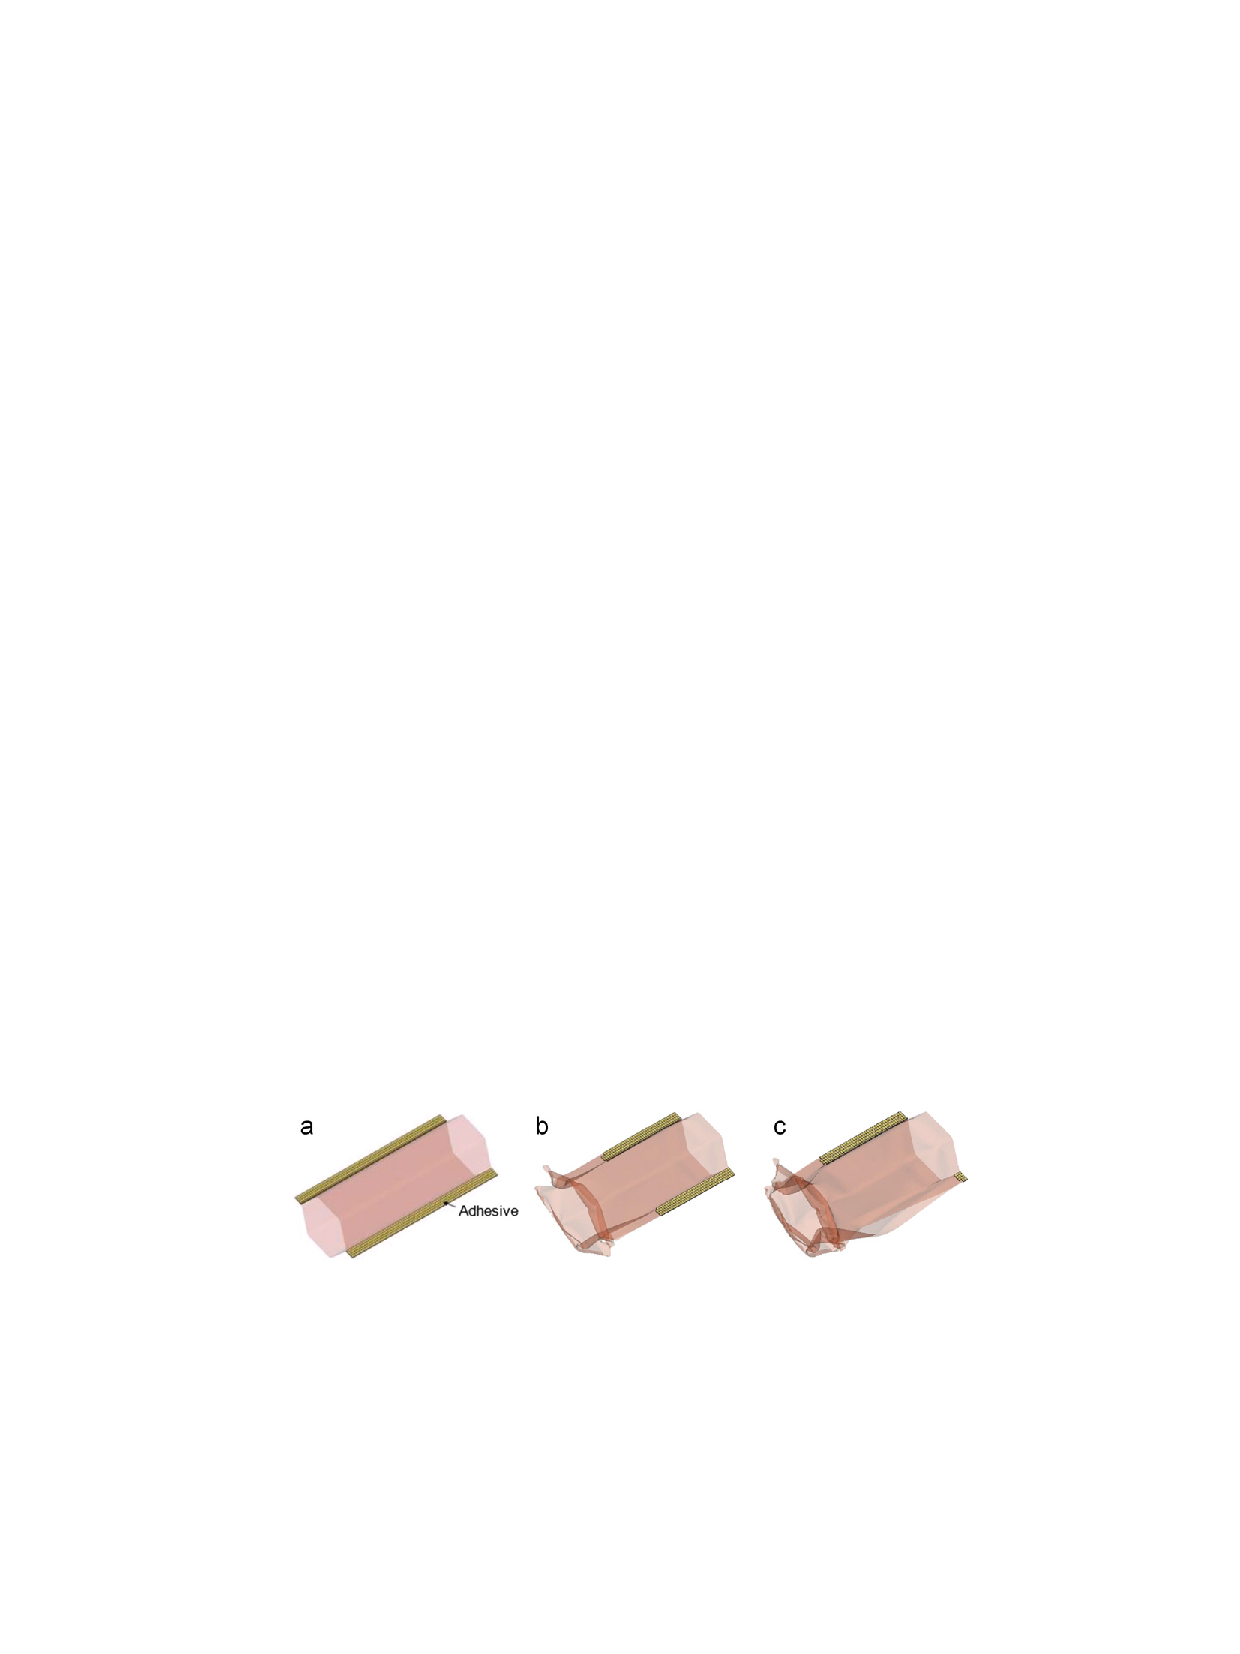
\includegraphics[width=0.9\linewidth]{IMG_CUTRES/yangs_tube}
	\caption[FEM analysis of a hexagonal crash box carried out by \cite{Yang2012}.]{FEM analysis of a hexagonal crash box carried out by \cite{Yang2012}. The begginning of tube's head opening can be seen on stage B, and it has totally peeled the adhesive layer by stage C.}
	\label{fig:yangs_tube}
\end{figure}

Using the scripting capabilities of the developed model, an hexagonal crash tube was tested. The collapse process of this section in the developed model is fairly prone to trigger missfunction, and it highly resembled the problems that \cite{Yang2012} found in the simulation.

% Insert figure & comment

This section aims to expose some of the most common critical situations found during the study development, usually by changing the boundary conditions affecting the tube. The reasons involved in this malfunctioning are related and always present combined, and were subducted by the addition of rivets and a stabilizing box to the model (\cref{sec:impact}).

\subsubsection{Triggering missfunctions}  % Head aperture
\label{sec:trig_missf}

Without the eventually included rivets, depending on the adherend thickness ---specifically for low values of this parameter---, triggering could not work properly: an excesive bending takes place at that point in the bonding flanges, together with little bending on points close to that part of the tube. In addition, this deformations happen to lead to opening the section.

This aperture may be caused either by a tendency to form waves with stiffer ---due to their undeformed state--- sections next to it which restrain this collapse mechanism on that point, or either by the presence of symmetrical wave patterns instead of parallel wave patterns leading to a wave in each adherend trying to open the section next to the trigger. Both situations may coexist, but either of them provokes the adhesive failure by pure mode I loading.

Failure may happen on the triggered cross section (see \cref{fig:trig_misf_A}, in this study, this was solved by using spot weld points in that cross section) or on the mid-tube (see \cref{fig:trig_misf_mid}). In this last case, general bending may also take place afterwards.

\begin{figure}
	\centering
	\begin{minipage}[b]{.65\linewidth}
		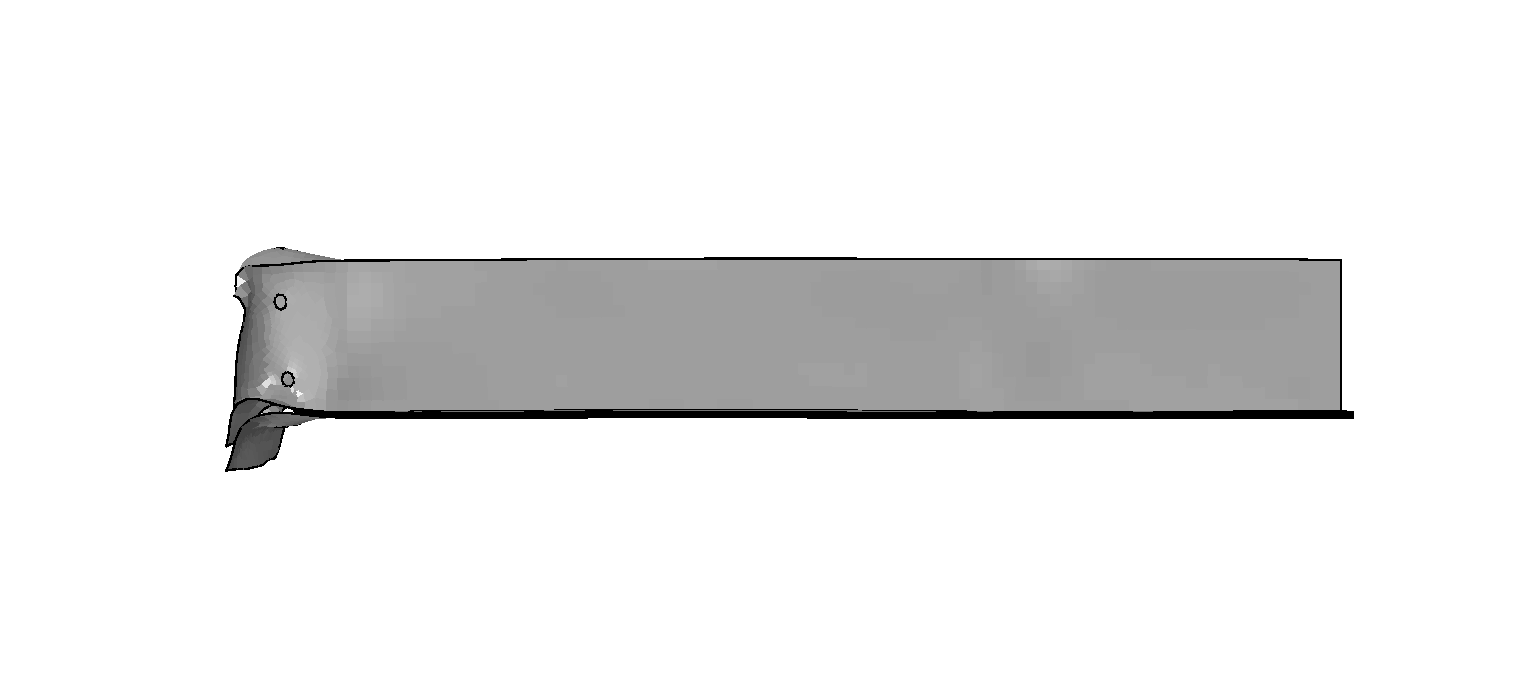
\includegraphics[width=\linewidth]{IMG_CUTRES/trig_misf_A1}
	\end{minipage}
	\quad
	\begin{minipage}[b]{.65\linewidth}
		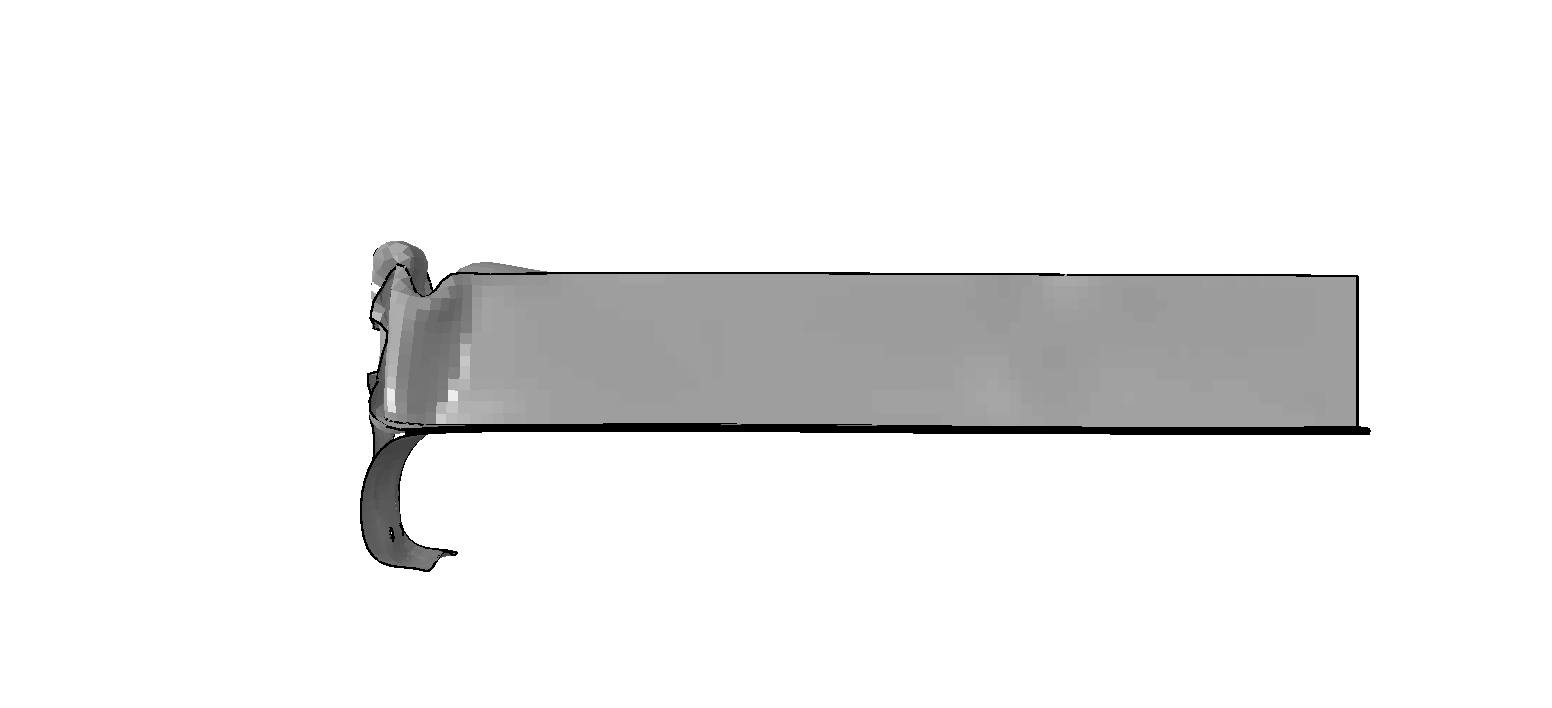
\includegraphics[width=\linewidth]{IMG_CUTRES/trig_misf_A2}
	\end{minipage}
	\quad
	\begin{minipage}[b]{.65\linewidth}
		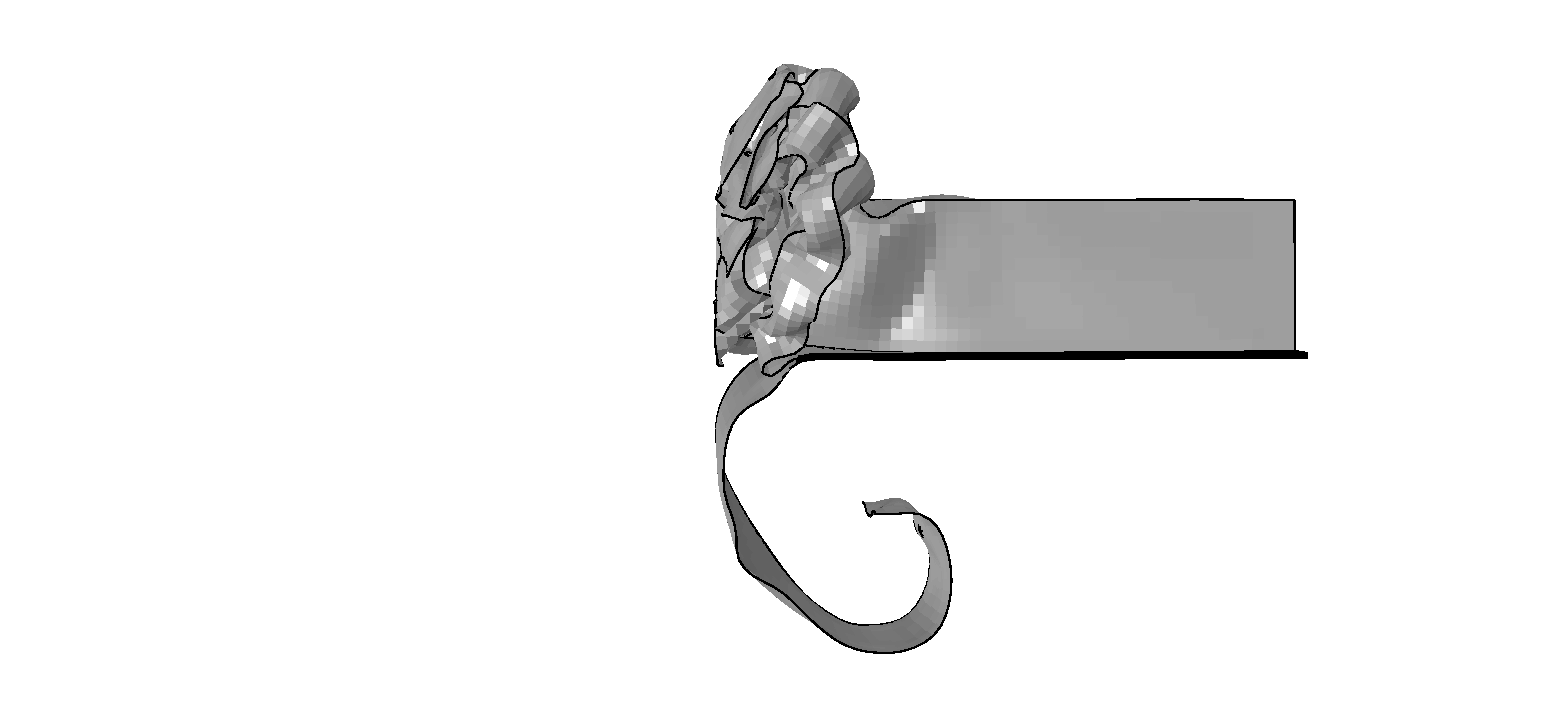
\includegraphics[width=\linewidth]{IMG_CUTRES/trig_misf_A3}
	\end{minipage}
	\caption{Trigger misfunction development on a top-hat section crash tube at $\SI{1.5}{\ms}$, $\SI{4.5}{\ms}$ and $\SI{15}{\ms}$.}
	\label{fig:trig_misf_A}
\end{figure}

\begin{figure}
	\centering
	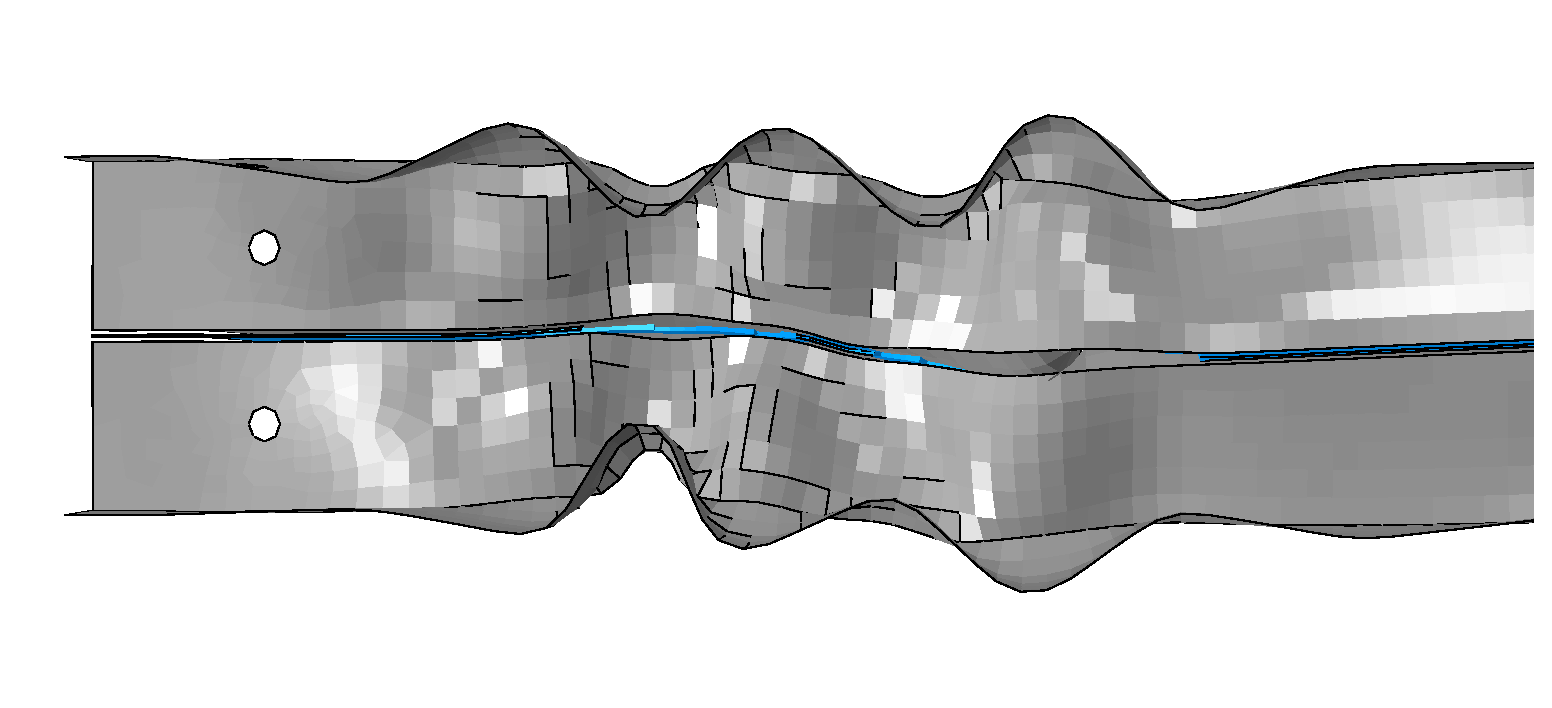
\includegraphics[width=0.7\linewidth]{IMG_CUTRES/trig_misf_mid}
	\caption[View cut detail of a double hat section crash tube with triggering misfunction initiation on a middle point.]{View cut detail of a double hat section crash tube with triggering misfunction initiation on a middle point. Focus on the symmetrical bending wave pattern. Adhesive in blue.}
	\label{fig:trig_misf_mid}
\end{figure}

%\begin{figure}
%	\centering
%	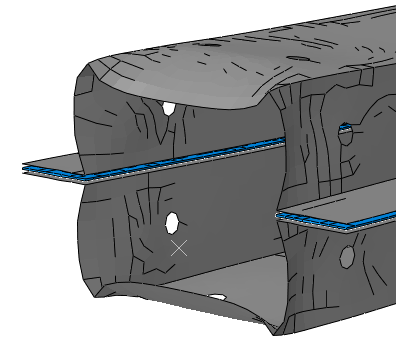
\includegraphics[width=.7\linewidth]{IMG_CUTRES/tmfB_detail}
%	\caption{Detail of a double hat section tube head in which triggering missfunction is starting to develop.}
%	\label{fig:tmfB_detail}
%\end{figure}

\begin{figure}
	\centering
	\begin{minipage}[b]{.22\linewidth}
		\centering
		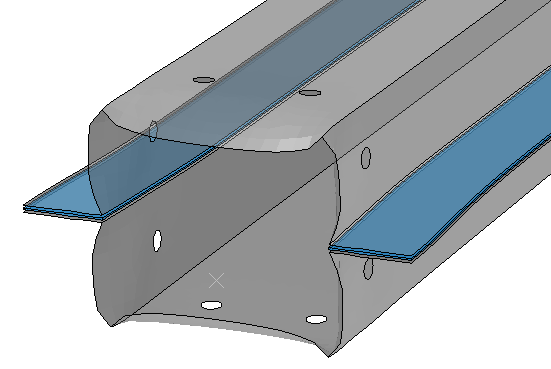
\includegraphics[width=\linewidth]{IMG_CUTRES/tmf1}
		$\SI{0.6}{\ms}$
	\end{minipage}
	\quad
	\begin{minipage}[b]{.22\linewidth}
		\centering
		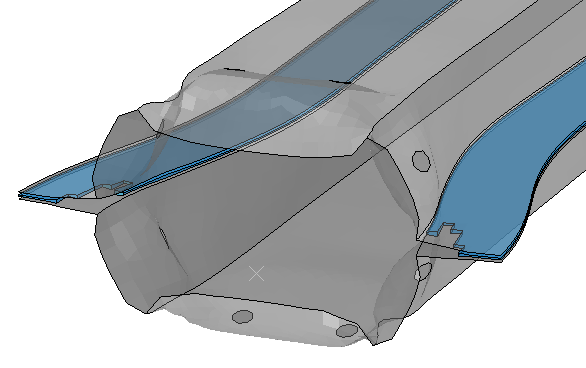
\includegraphics[width=\linewidth]{IMG_CUTRES/tmf2}
		$\SI{1.05}{\ms}$
	\end{minipage}
	\quad
	\begin{minipage}[b]{.22\linewidth}
		\centering
		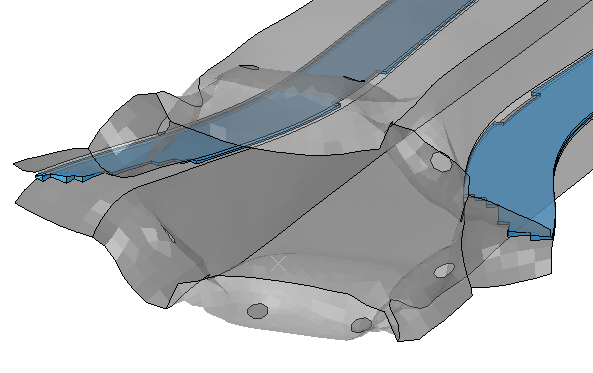
\includegraphics[width=\linewidth]{IMG_CUTRES/tmf3}
		$\SI{1.5}{\ms}$
	\end{minipage}
	\quad
	\begin{minipage}[b]{.22\linewidth}
		\centering
		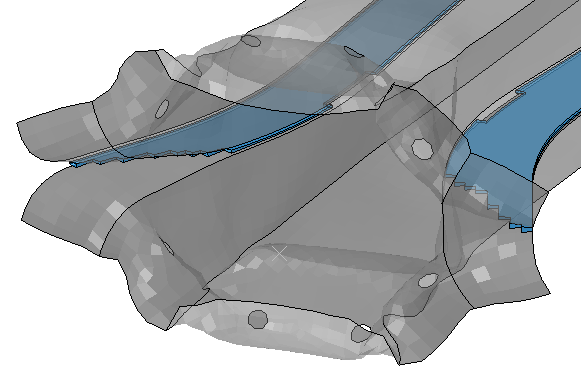
\includegraphics[width=\linewidth]{IMG_CUTRES/tmf4}
		$\SI{1.95}{\ms}$
	\end{minipage}
	\caption[Triggering missfunction development process on a double hat section crash tube.]{Triggering missfunction development process on a double hat section crash tube. Adhesive in blue.}
	\label{fig:tmf}
\end{figure}

By facing \cref{fig:tmf}, it is supposed that this situation has its origin on an adherend thickness-triggering relation that also depends on the cross section of the tube, as the plates initial bend is allowed by the reduced adherend thickness and this is the origin of the peeling failure due to the plates bending directionality, which tends to open the union from the inside. After this situation has started, the more the head is deformed, the more it is developed. There are several other arguments supporting this theory:
\begin{itemize}
	\item The lack of triggering also leads to this situation.

	\item Hexagonal cross sections \cite{Yang2012} are particulary prone to develop this critical situation.

	\item Thicker adherends seem to be about of avoiding this misfunction before starting other critical collapse mechanisms.

	\item It is the main critical situation that can be found on top-hat cross section crash tubes.
\end{itemize}

\Cref{fig:tmf_fd} shows the corresponding force-displacement curve of the tube of \cref{fig:tmf}. In this critical situation, adherends start to bend over a certain point of the tube provoking the peeling along the tube in the process. The second peak present in \cref{fig:tmf_fd} may be motivated by the impact plate reaching this bending point and thus starting an in-plane compression of the adherends like the experienced in the beginning.

\begin{figure}
	\centering
	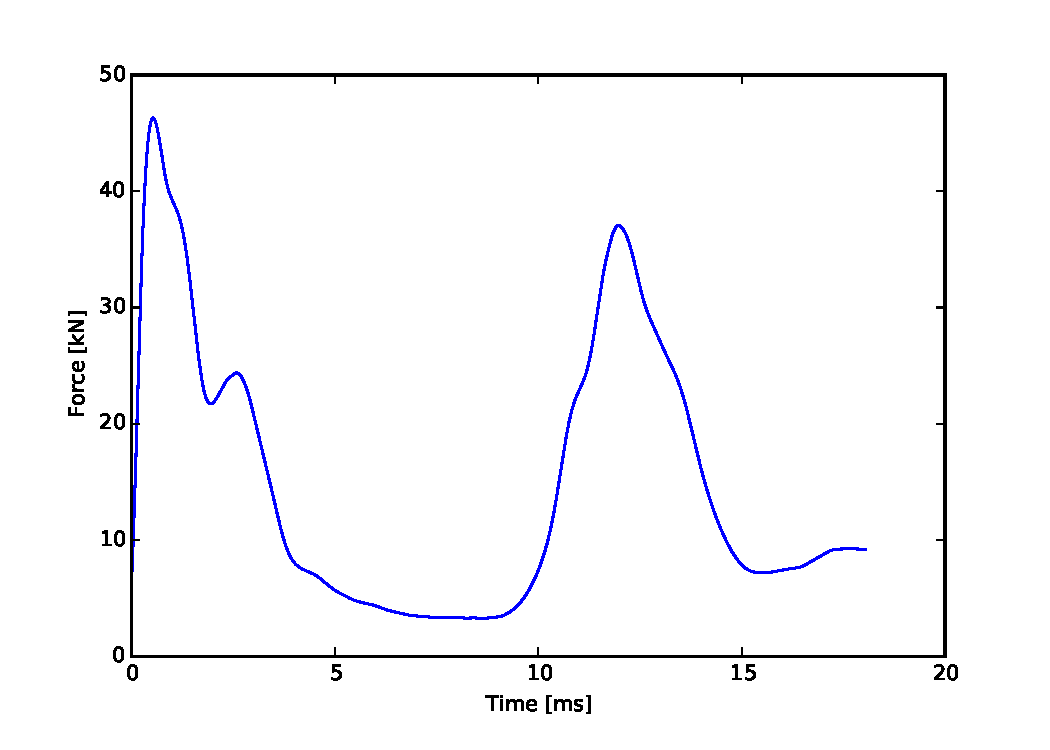
\includegraphics[width=0.7\linewidth]{IMG_CUTRES/tmf_fd}
	\caption{Force-displacement curve for a crash tube with triggering missfunction.}
	\label{fig:tmf_fd}
\end{figure}

This misfunction is also particularly independent of the tube length, as the analysis with different values of this parameter showed. This situation is also particularly easy to be developed on hexagonal crash boxes, as \cref{fig:hex_tmf} shows.

\begin{figure}
	\centering
	\begin{minipage}[b]{.3\linewidth}
		\centering
		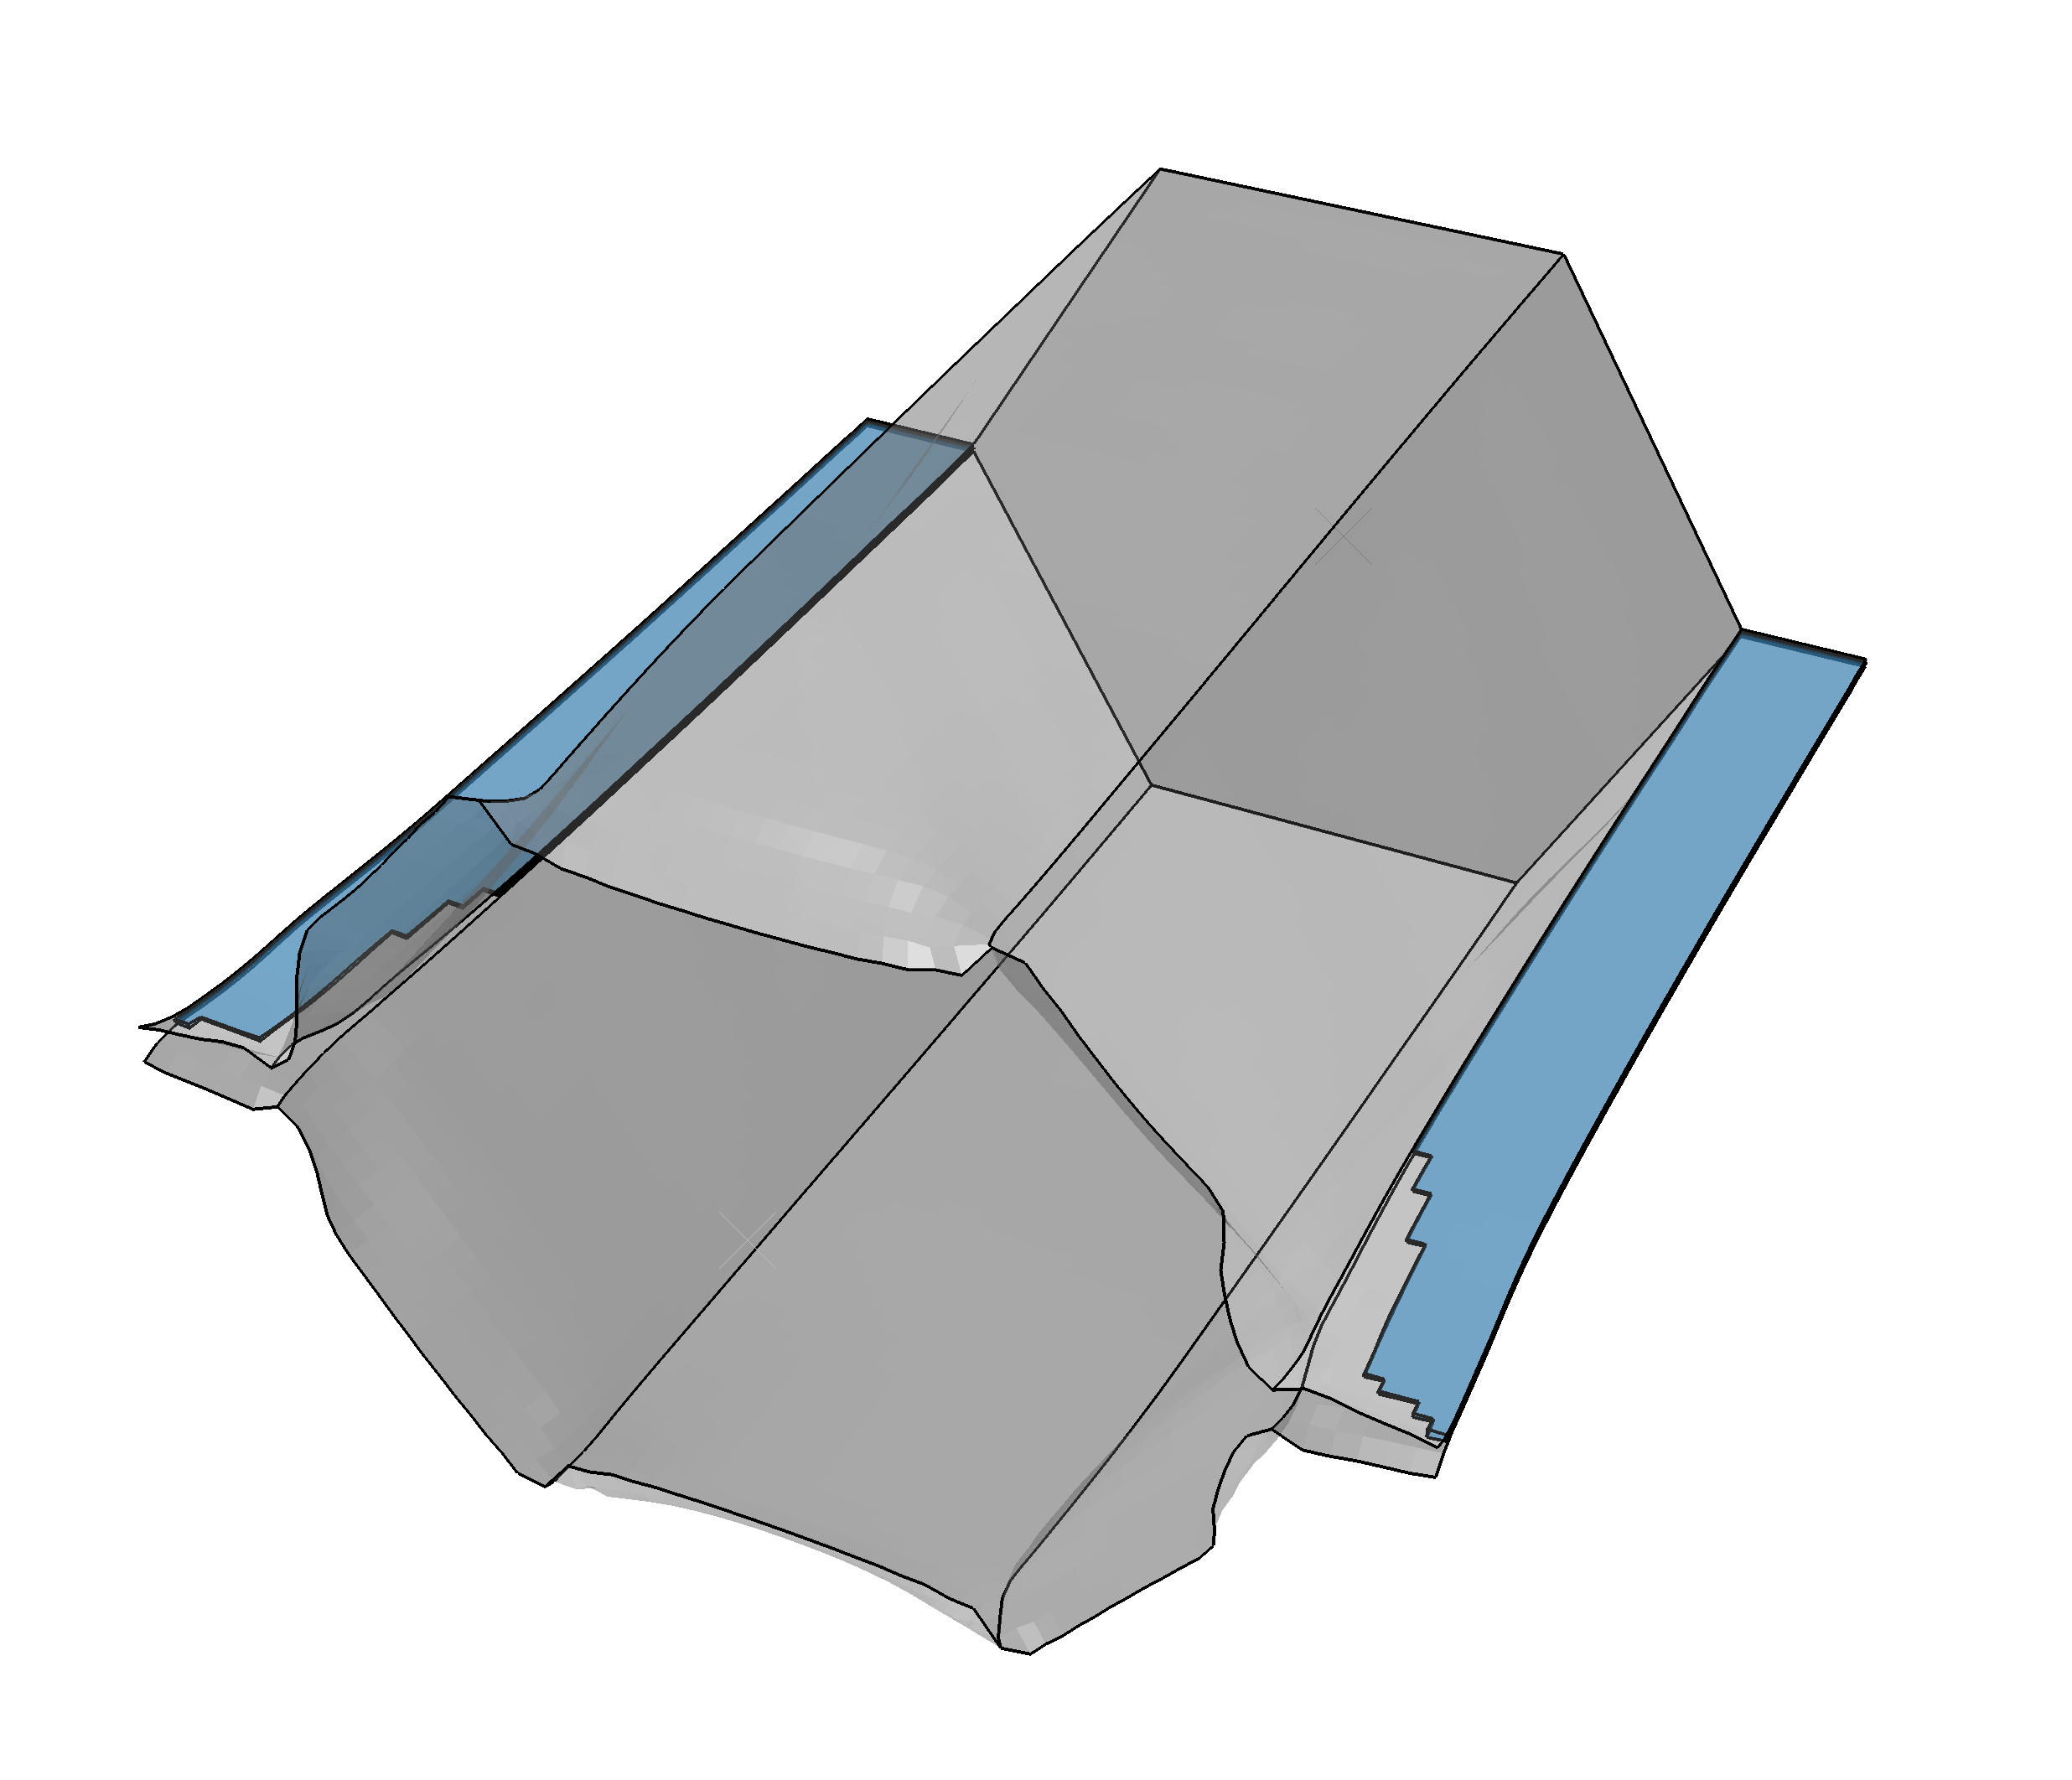
\includegraphics[width=\linewidth]{IMG_CUTRES/hex1}
		$\SI{0.6}{\ms}$
	\end{minipage}
	\quad
	\begin{minipage}[b]{.3\linewidth}
		\centering
		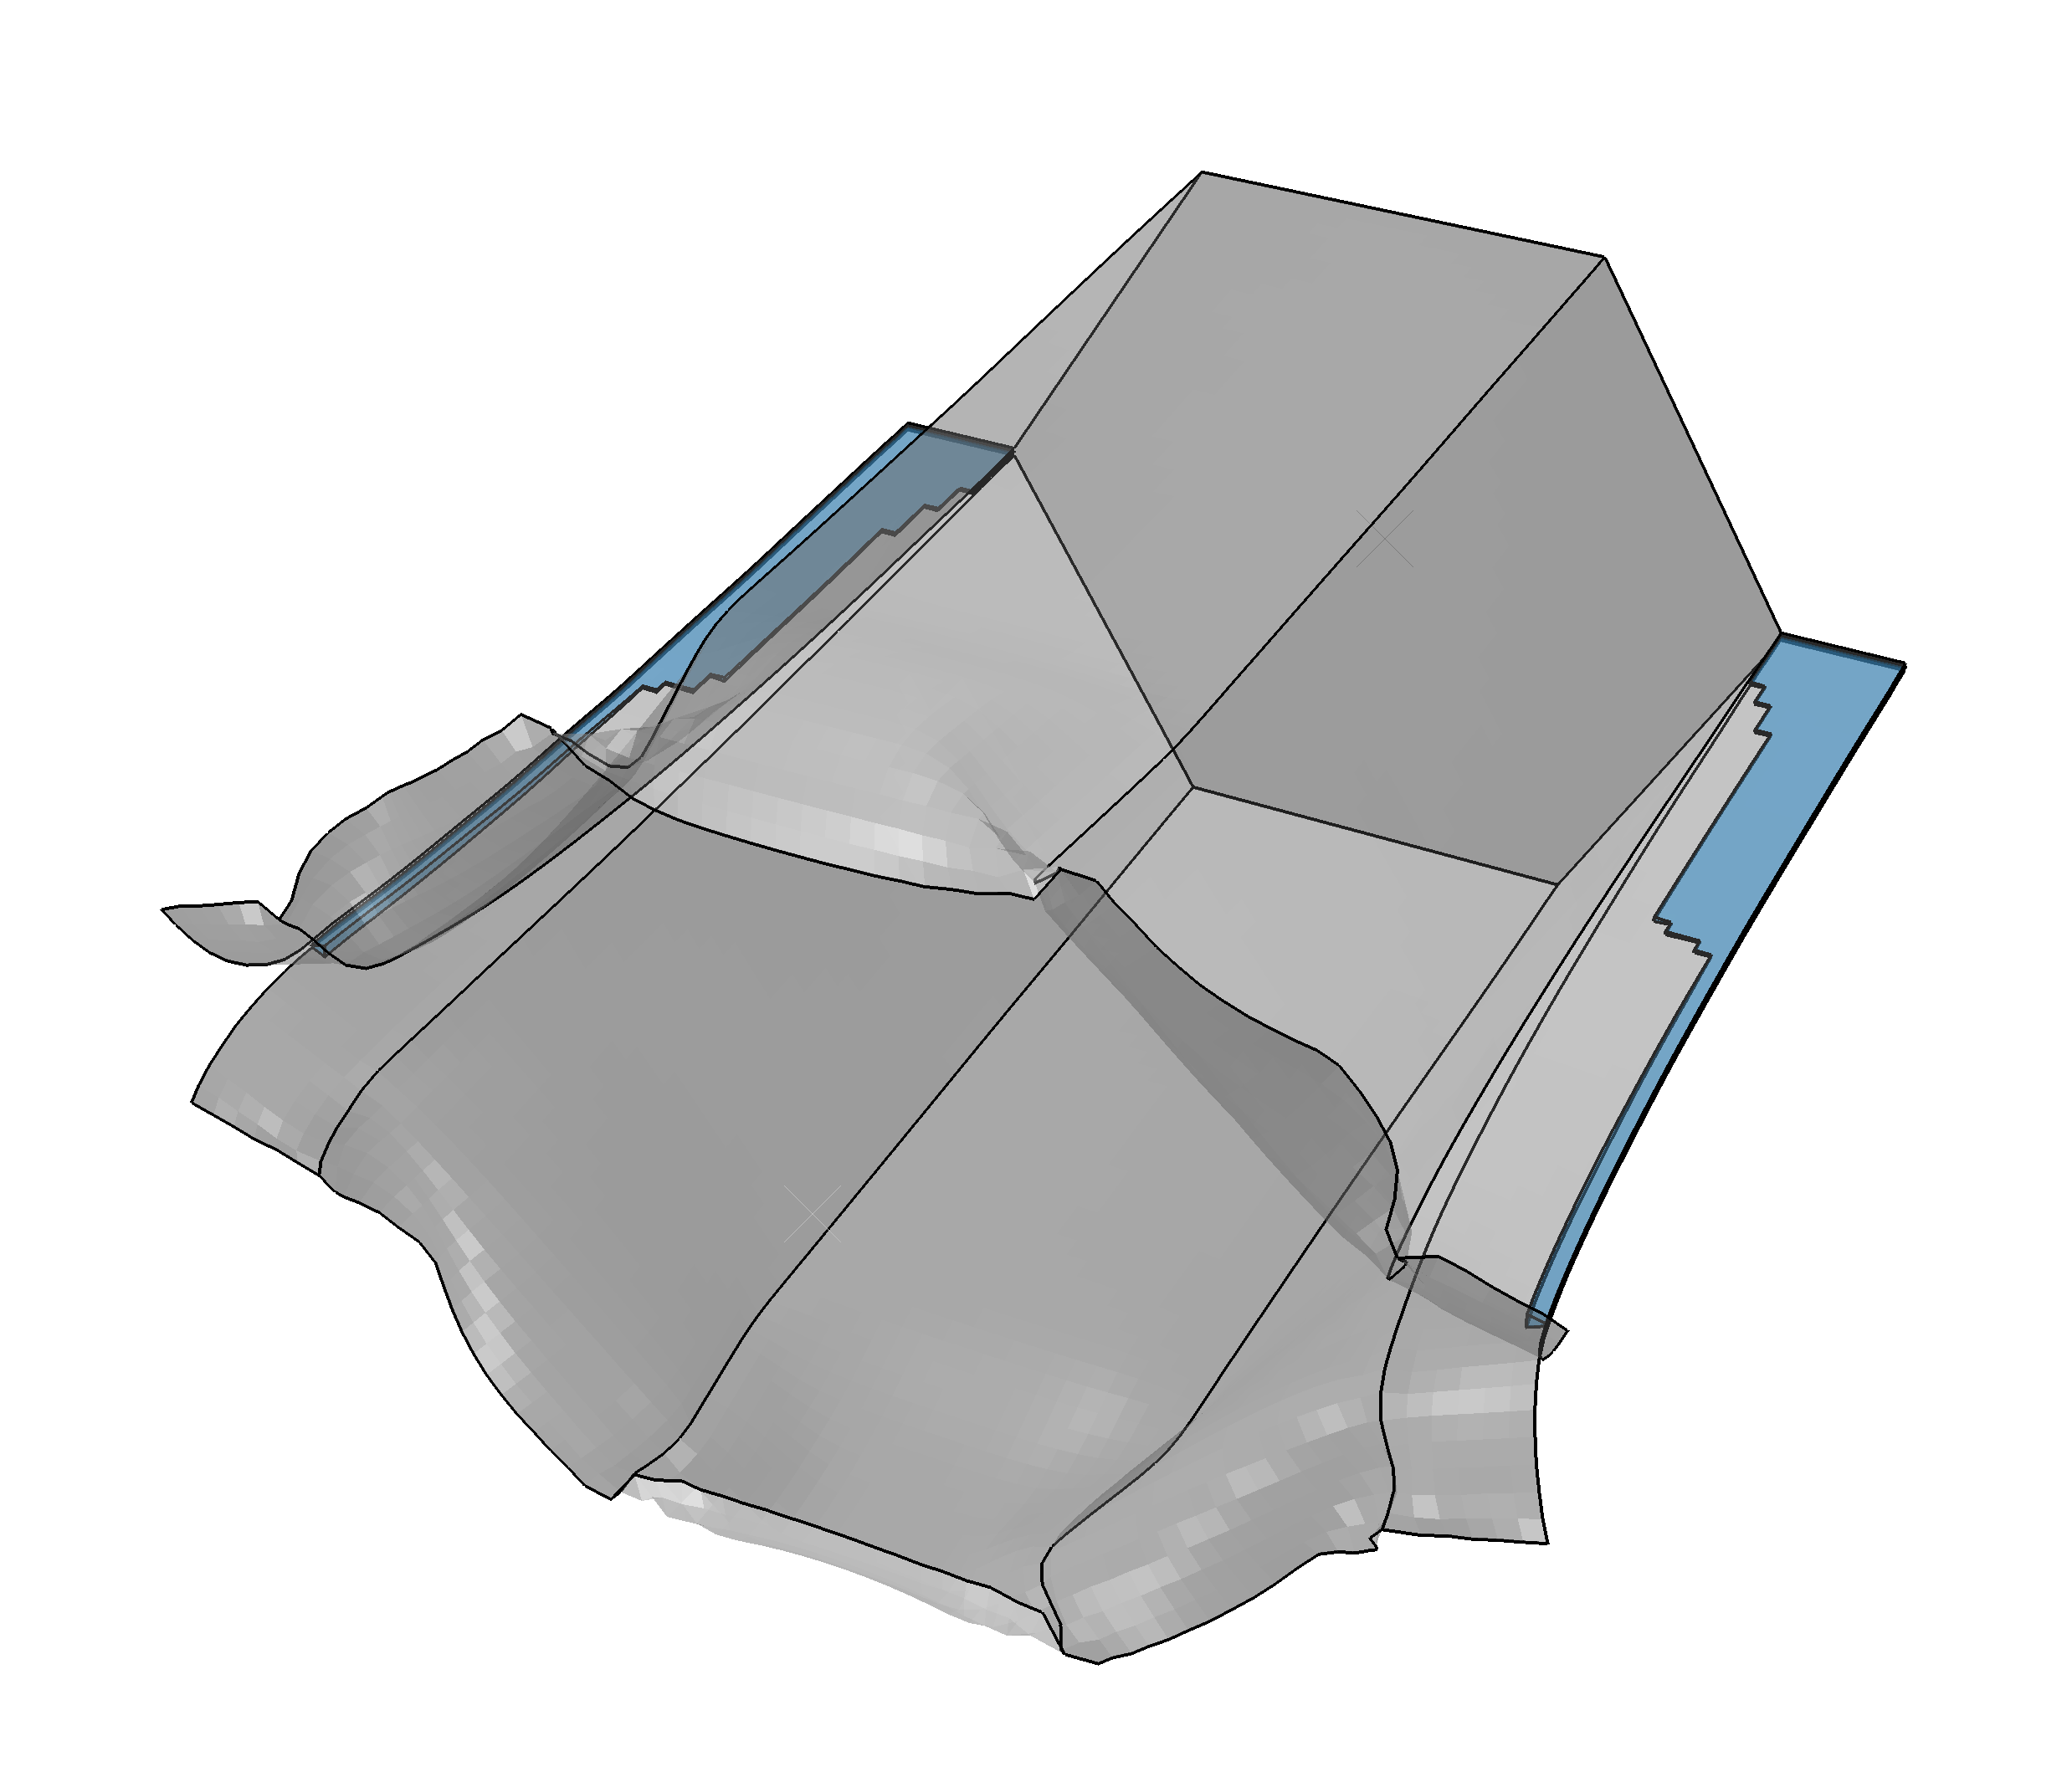
\includegraphics[width=\linewidth]{IMG_CUTRES/hex2}
		$\SI{1.2}{\ms}$
	\end{minipage}
	\quad
	\begin{minipage}[b]{.3\linewidth}
		\centering
		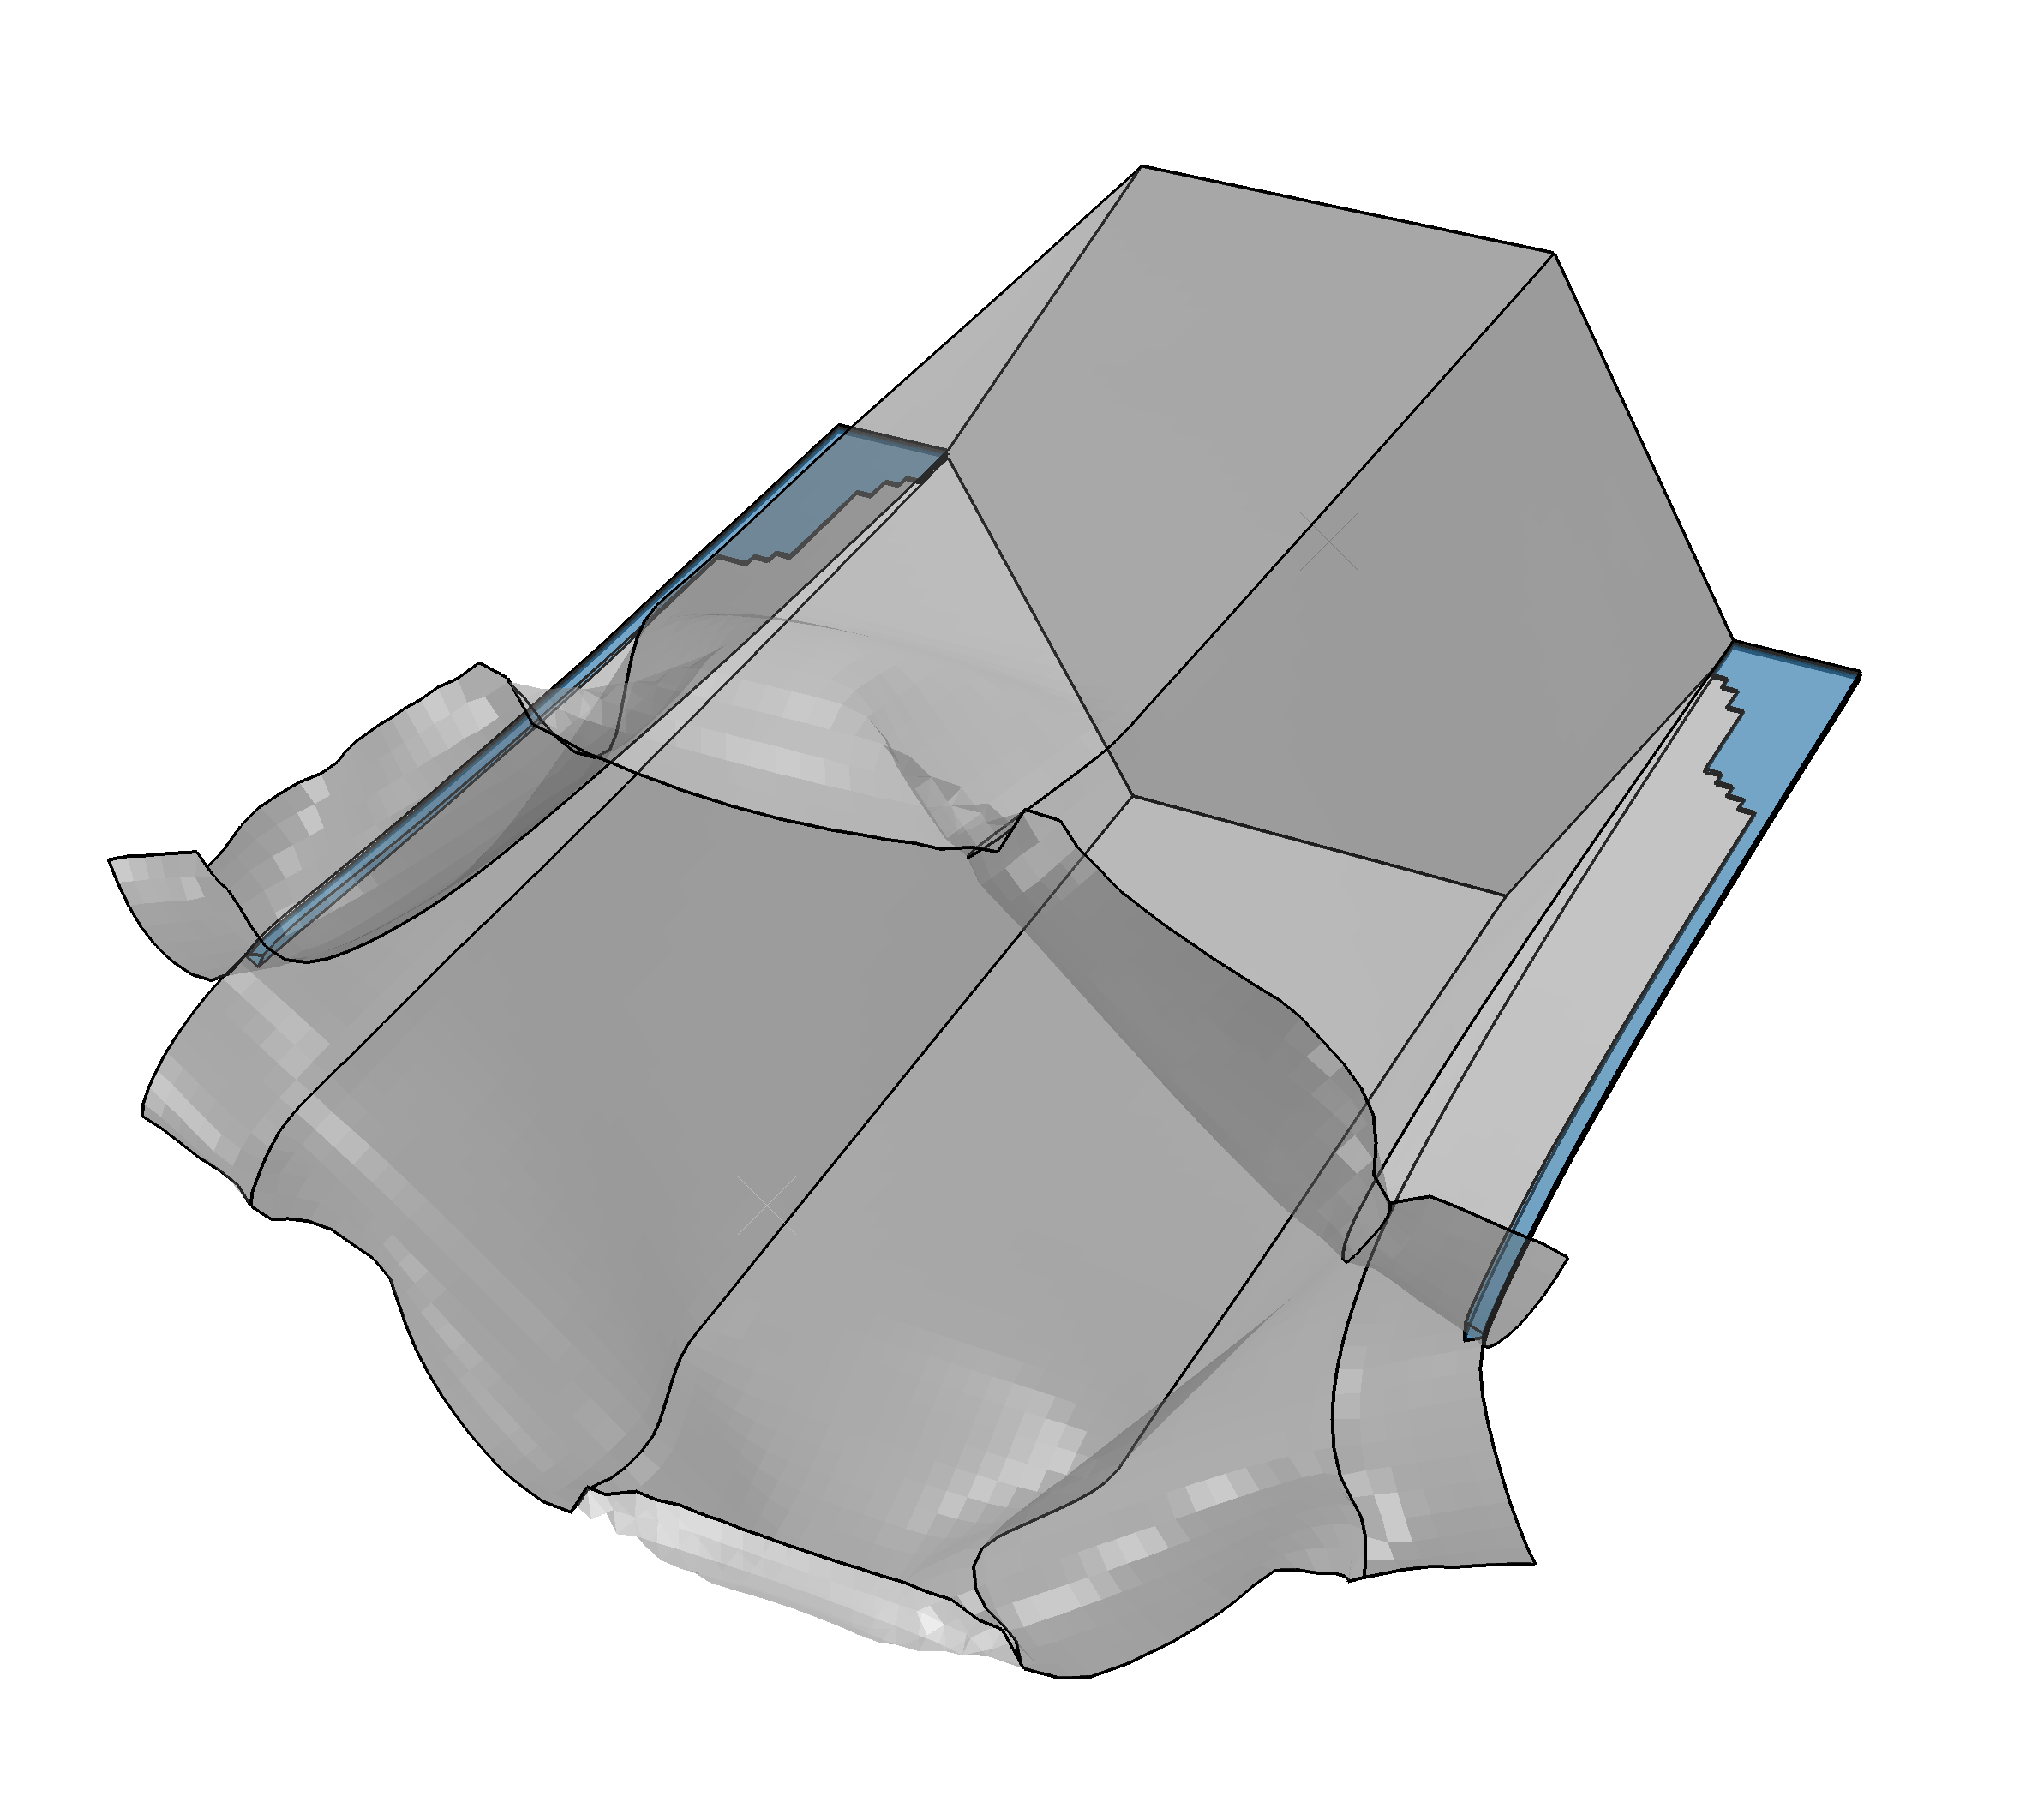
\includegraphics[width=\linewidth]{IMG_CUTRES/hex3}
		$\SI{1.8}{\ms}$
	\end{minipage}
	\caption[Triggering missfunction development process on a hexagonal cross section crash tube.]{Triggering missfunction development process on a hexagonal cross section crash tube. Adhesive in blue.}
	\label{fig:hex_tmf}
\end{figure}

\subsubsection{General bending}

It was found that in many cases, during the wave formation process, a minor difference between plates deformation, eventually resulted in the box bending by some mid-point, diverting the tube's directrix instead of crushing the device in a straight direction (see \cref{fig:general_bending}).

\begin{figure}
	\centering
	\begin{minipage}[b]{.7\linewidth}
		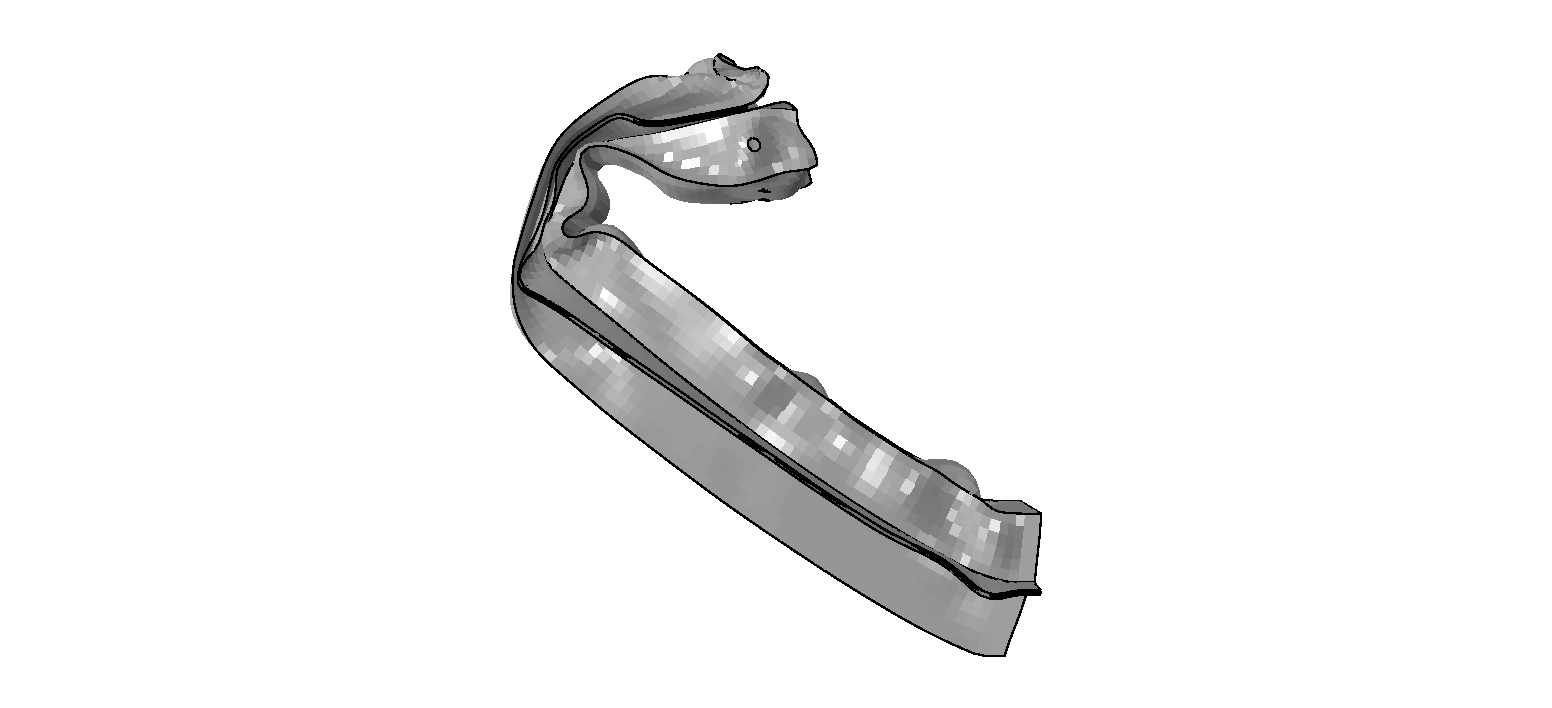
\includegraphics[width=\linewidth]{IMG_CUTRES/general_bending_73}
	\end{minipage}
	\quad
	\begin{minipage}[b]{.3\linewidth}
		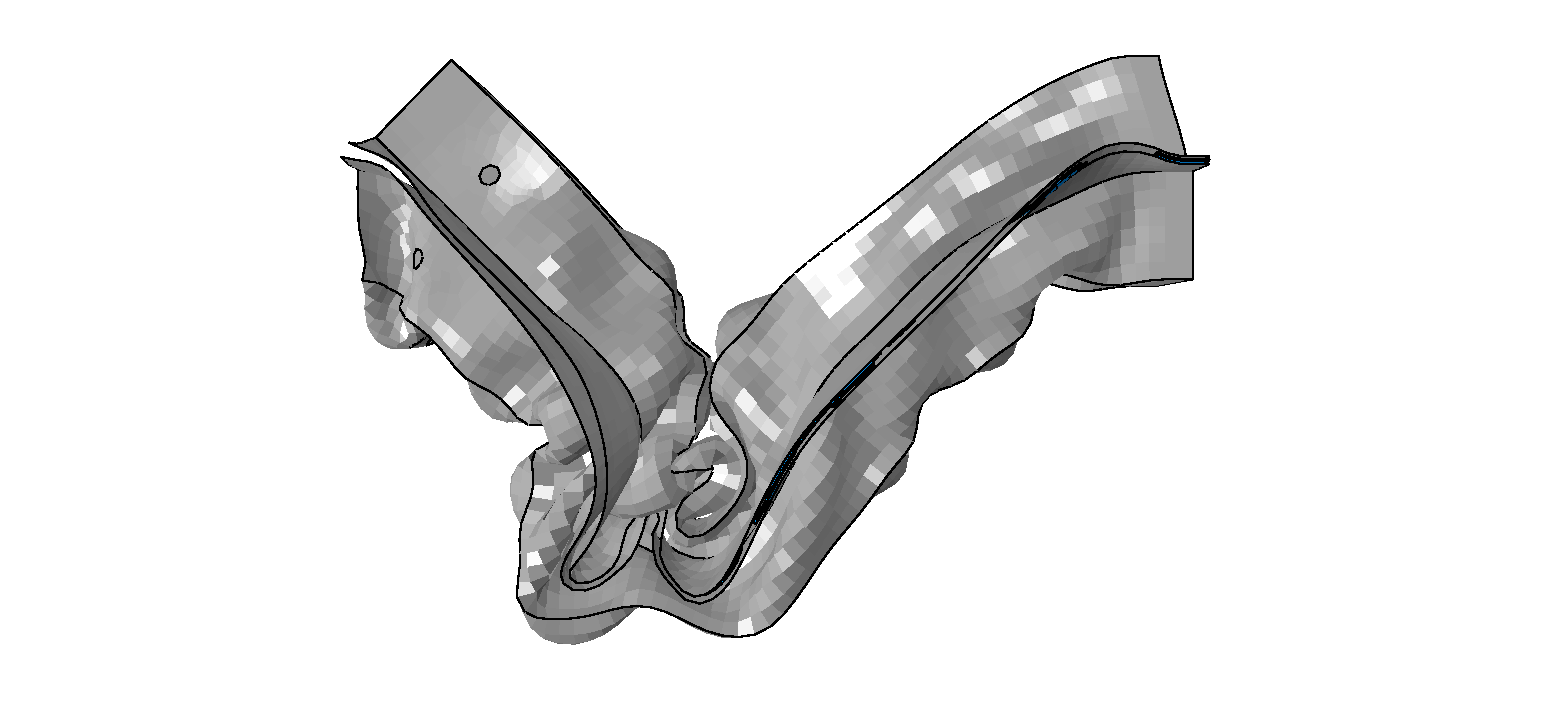
\includegraphics[width=\linewidth]{IMG_CUTRES/general_bending_48}
	\end{minipage}
	\quad
	\begin{minipage}[b]{.3\linewidth}
		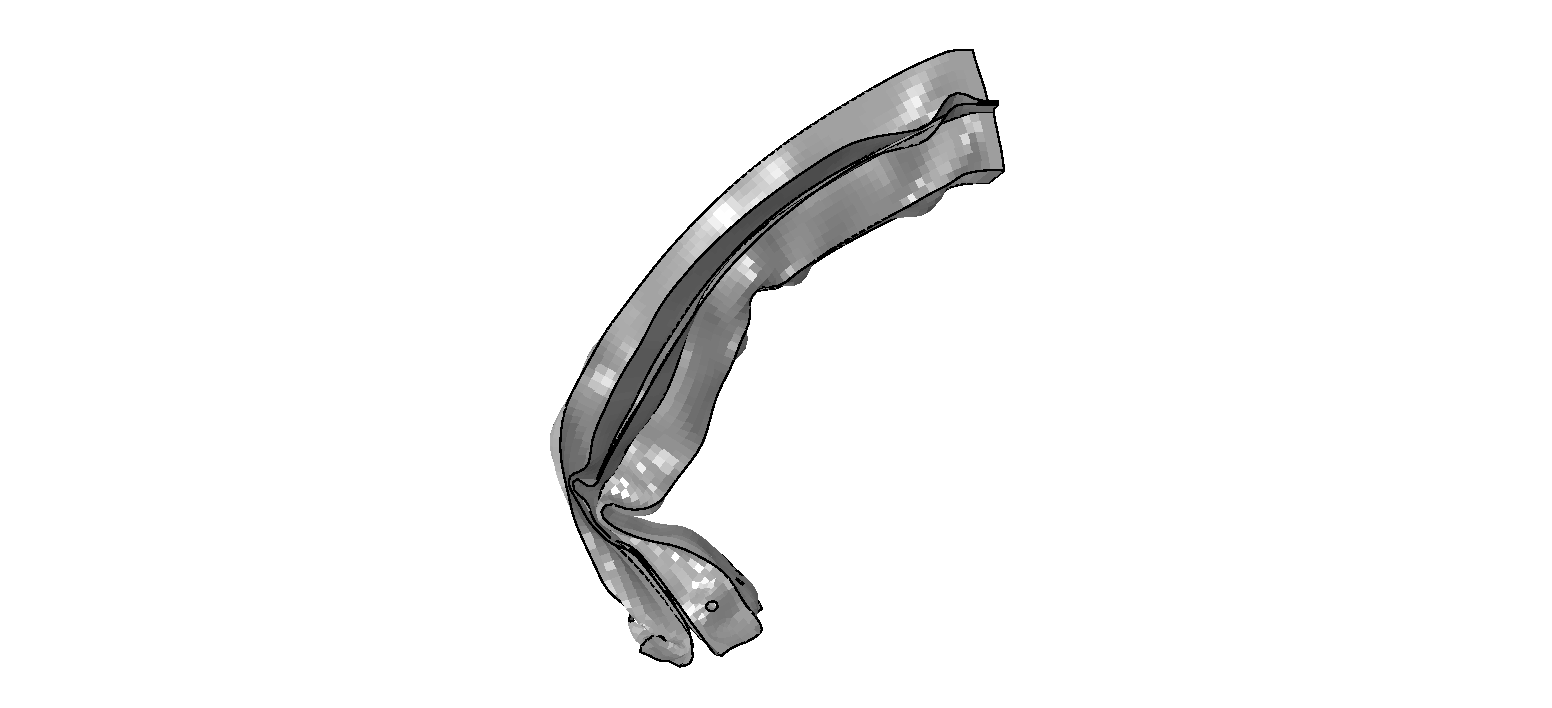
\includegraphics[width=\linewidth]{IMG_CUTRES/general_bending_72}
	\end{minipage}
	\quad
	\begin{minipage}[b]{.3\linewidth}
		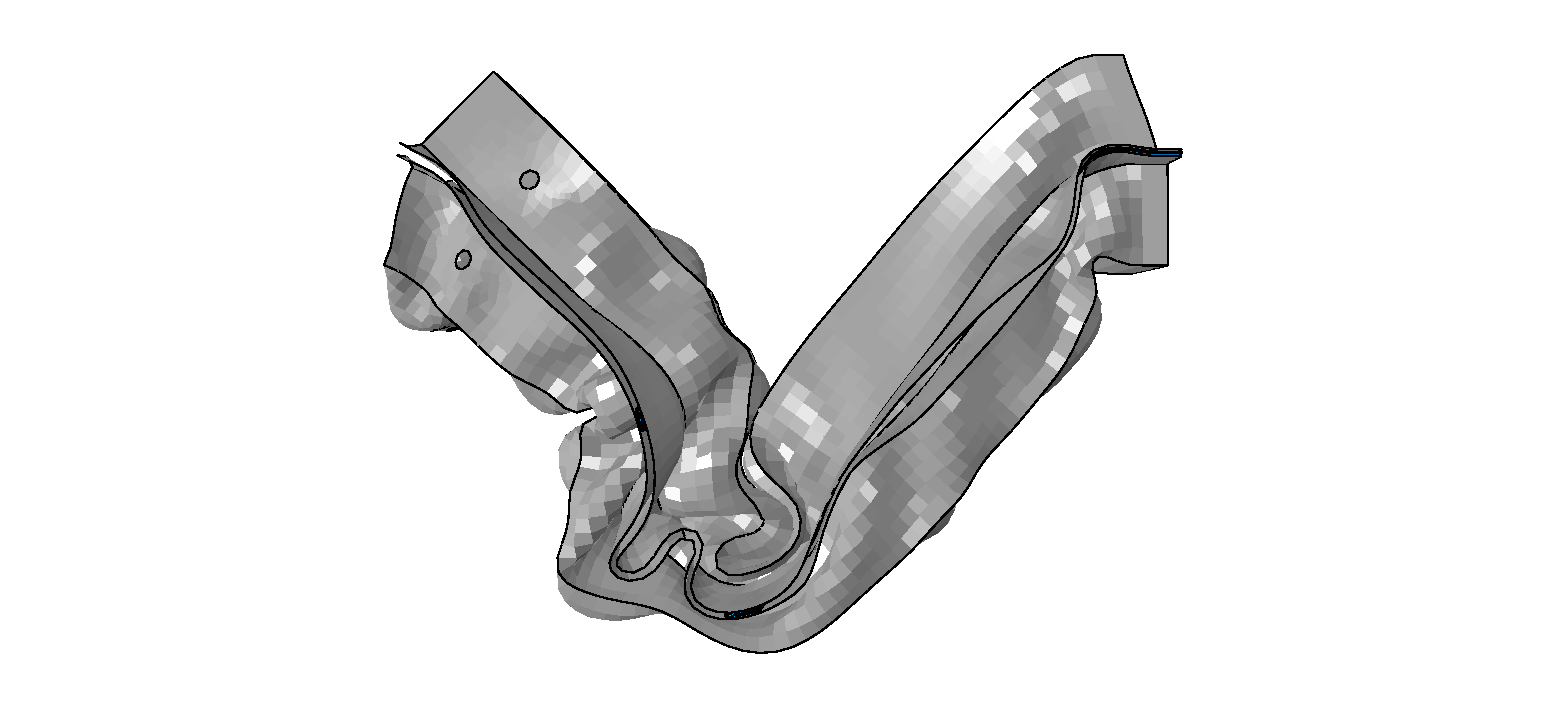
\includegraphics[width=\linewidth]{IMG_CUTRES/general_bending_55}
	\end{minipage}
\caption[Final deformation status of a double hat section crash tube model without stabilizing box in a general bending critical situation.]{Final deformation status of a double hat section crash tube model without stabilizing box in a general bending critical situation. Crushing from the left.}
\label{fig:general_bending}
\end{figure}

Analyzing the origin of this situation, several possible reasons were considered:
\begin{itemize}
	\item A longer wave on one side, followed by a less pronounced one. Membrane effect on the former one makes it a stiffer point. The last one is a weak section, as the consecutive adherend planes are folding together. As this situation only takes place on one of the adherends, the faux-symmetry ceases to exist, thus bending the tube by some mid-point.

	\item Following a behaviour similar to that one found in triggering missfunction, aperture of the section happens in some mid-point. Usually an excesively opened wave by the union plane, sided by two under-formated waves that cannot compensate the aperture, triggers this failure.
\end{itemize}

This situation usually takes place with minor adhesive failure on its initial phases, and rapidly failing in a peel-shear combination when the bend is completely formed on almost the whole surface.

Ideal bonding ---using tie constraints instead of a material union--- presented this collapse mechanism, only differing in the last phases, depicted in \cref{fig:general_bending}, in which the adhesive fails.

This suggests that the adhesive meets its objective on retainning the two flanges together, at least until the critical failure has completely developed itself, and thus suggesting an adherend or trigger origin of this problem.

It also suggests that the adhesive influence on the general response is of little importance on the last phases, meaning that once the critical situation is initiated, the response barely depends on the bond.

On the other hand, top-hat section crash tubes were found to be fairly more resistant to developing this kind of malfunction, as no cases were found.

\subsubsection{General peeling due to plates buckling}

Excessively thick adherend plates prevent wave formation, resulting in other collapse mechanisms development, such as a buckling-like deformation, as a slender beam subjected to high compression. In this situation, each plate bends to a side, peeling the union in the process. In this situation, the stiffness difference between adherend and adhesive results in a behavior that could be described as if the former imposed deformations to the later.

Although it could not be measured, it is supposed that a big share part of the Ea value comes from elastic-plastic deformation of the adherend plates. The adhesive failure is purely mode I, and thus only the corresponding fracture energy is absorbed, which is recalled that was about one fifth of the other modes value. In spite of that, SEA values with $\SI{2}{\mm}$ plate thickness were close to the ones found with $\SI{1}{\mm}$ carried out by \cite{Peroni2009} with a stable collapse mechanism.

\begin{figure}
	\centering
	\begin{minipage}[b]{.48\linewidth}
	\centering
	\begin{minipage}[b]{\linewidth}
		\centering
		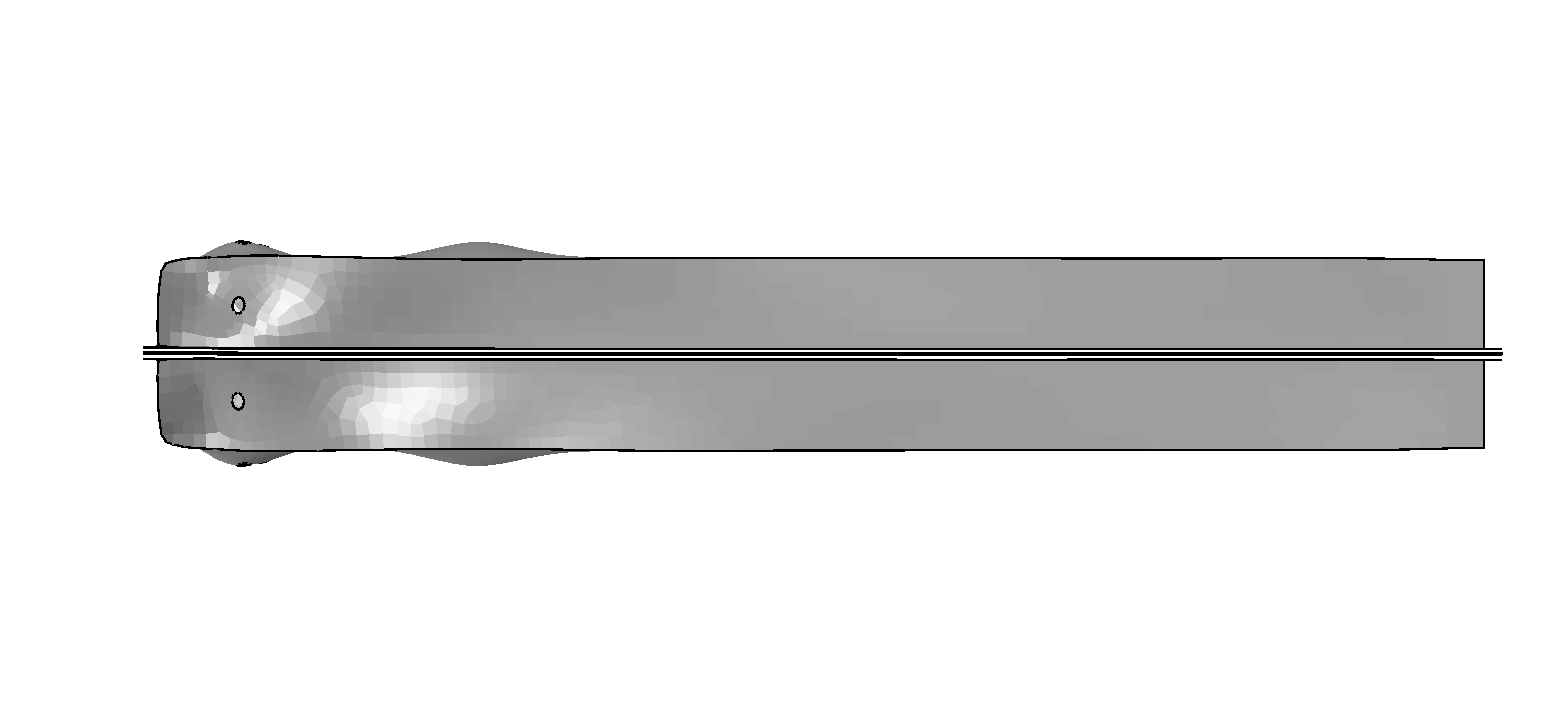
\includegraphics[width=\linewidth]{IMG_CUTRES/gppb67}
		$\SI{2.0}{\ms}$
	\end{minipage}
	\quad
	\begin{minipage}[b]{\linewidth}
		\centering
		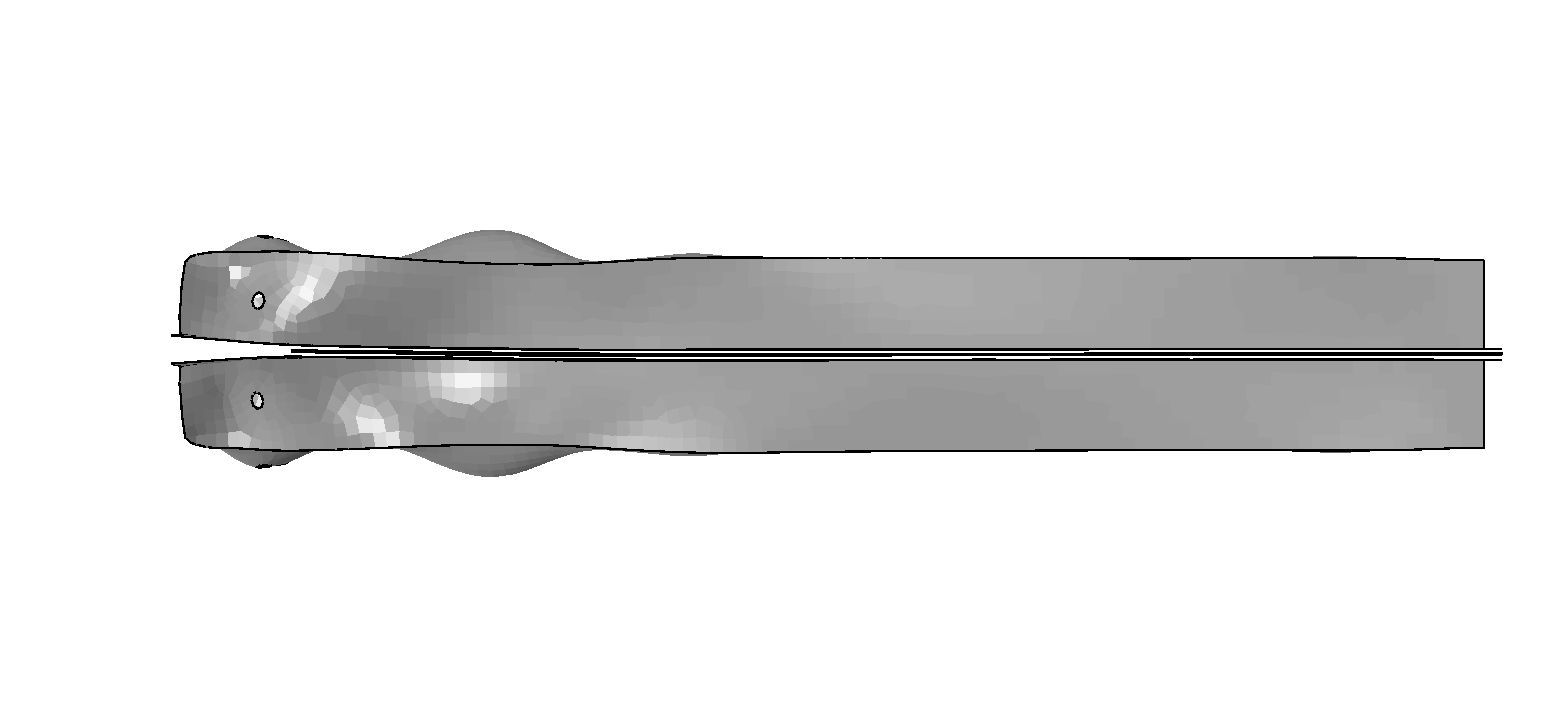
\includegraphics[width=\linewidth]{IMG_CUTRES/gppb84}
		$\SI{2.5}{\ms}$
	\end{minipage}
	\quad
	\begin{minipage}[b]{\linewidth}
		\centering
		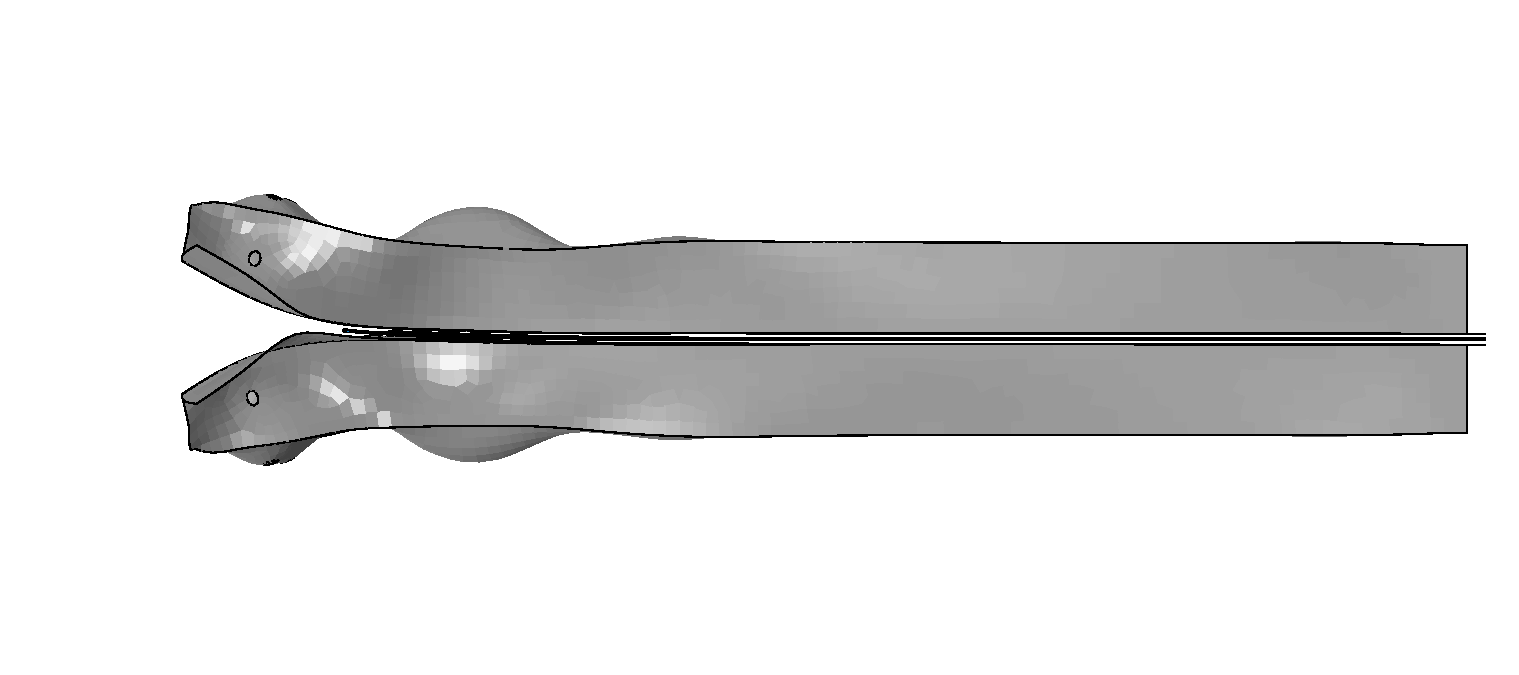
\includegraphics[width=\linewidth]{IMG_CUTRES/gppb100}
		$\SI{3.0}{\ms}$
	\end{minipage}
	\end{minipage}
	\quad
	\begin{minipage}[b]{.48\linewidth}
		\centering
		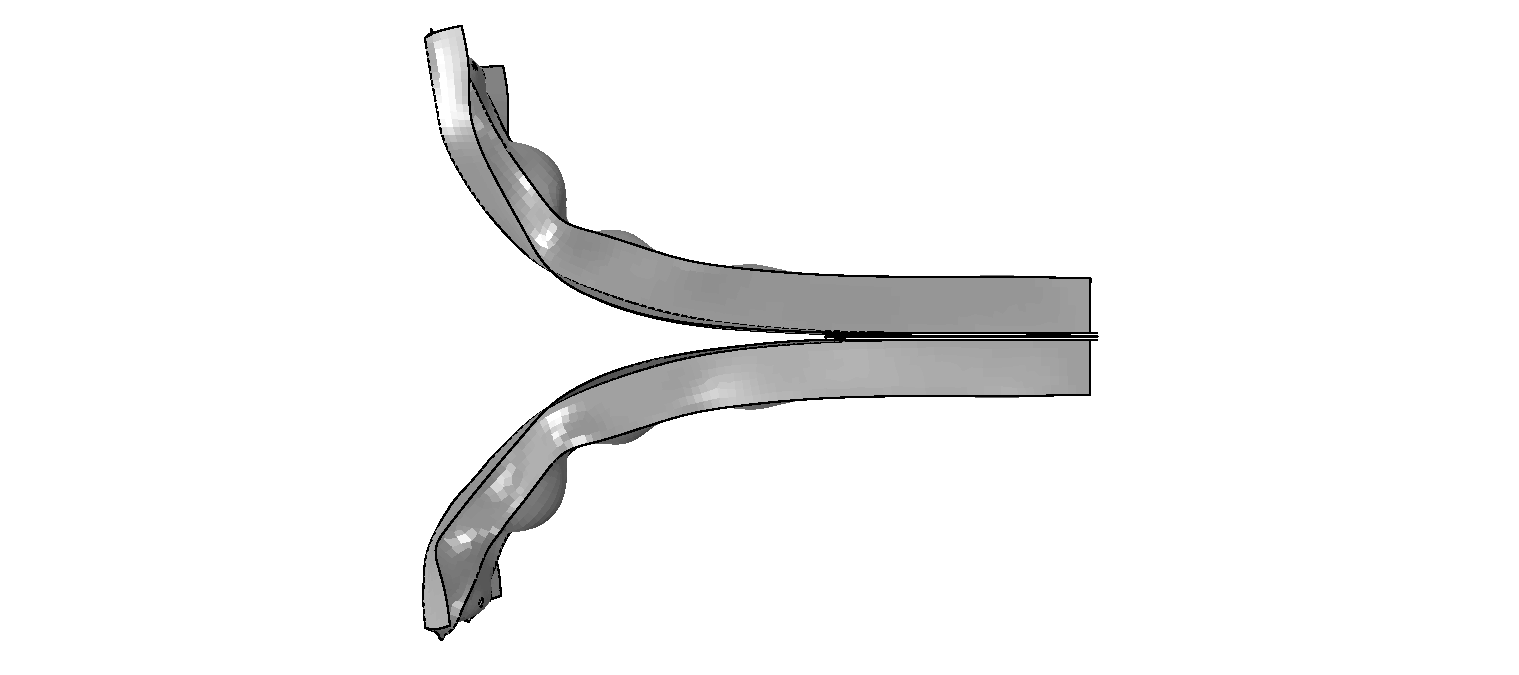
\includegraphics[width=\linewidth]{IMG_CUTRES/gppb300}
		$\SI{9.0}{\ms}$
	\end{minipage}

	\caption{General peeling due to plates buckling collapse process.}
	\label{fig:gppb}
\end{figure}

This fact may be used as an argument to make the adherends thicker, but the Pk was also strongly increased to over $\SI{100}{\kN}$ in this case as it can be seen on \cref{fig:gppb_fd}, which is undesirable. In that same figure, it can be seen how the pure mode I failure of the whole adhesive allows little energy absorption. SEA is $\SI{4.28}{\kJ/\kg}$, lower than other solutions due to this inefficiency.

\begin{figure}
	\centering
	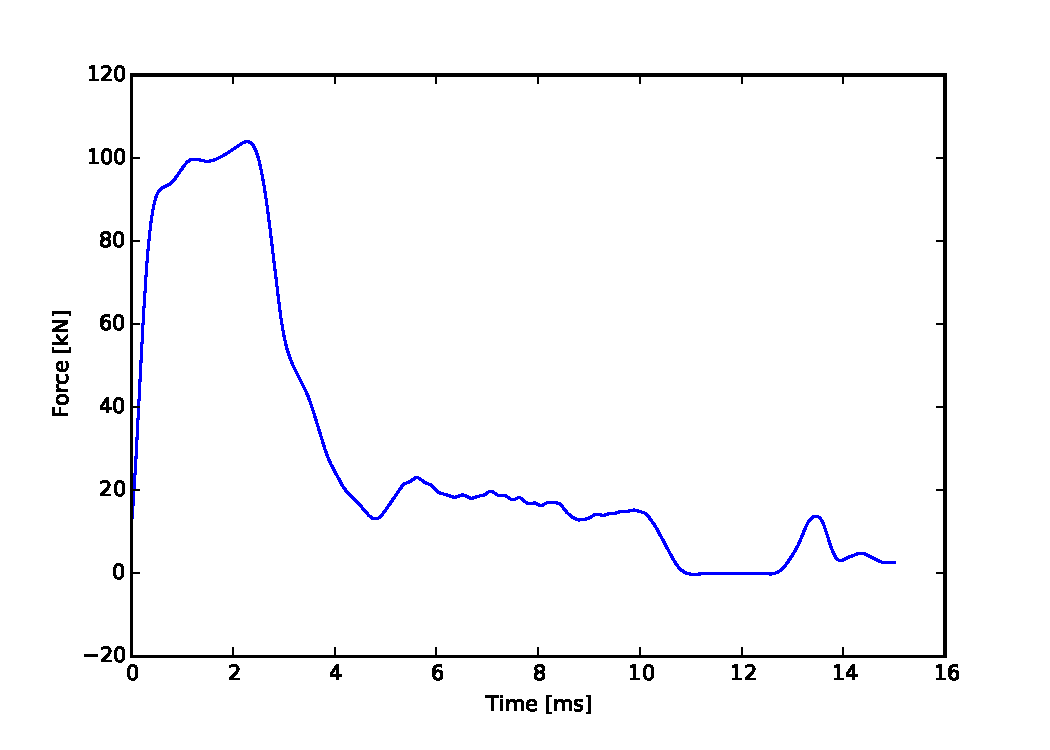
\includegraphics[width=0.7\linewidth]{IMG_CUTRES/gppb_fd}
	\caption{F-D for a $\SI{2}{\mm}$ adherend thick in which general peeling due to plates buckling is developed.}
	\label{fig:gppb_fd}
\end{figure}

Unlike the commented triggering missfunction, general peeling finds its origin on a buckling-like behavior of the plates which produces the peeling, while the malfunction of the trigger leads to local failure of the bonding, leading to the rotation of a part of the plate around a wave formed in a rearer point of the tube. In addition, triggering missfunction is easier to develop with lower thickness values, while general peeling is produced with higher values of this parameter.

\section{Interpretation}  % Include different geoms comparation if possible
\label{sec:interpretation}

In general terms, top-hat section tubes better resemble the reference crash boxes, specially due to their higher resistance to develop undesired collapse mechanisms.

\subsection{Stable collapse mechanism}

\Cref{fig:stable} depicts the collapse sequence of a top-hat crash tube, showing a stable crushing pattern. Analyzing the modeling, it can be concluded that this collapse was achieved thanks the stabilizing box, as it retains the plates at certain points. \Cref{fig:stabil_box} depicts the final state of the crushing process, showing how the stabilization box retained the crash tube.

\begin{figure}
	\centering
	\begin{minipage}[b]{.06\linewidth}
		\centering
		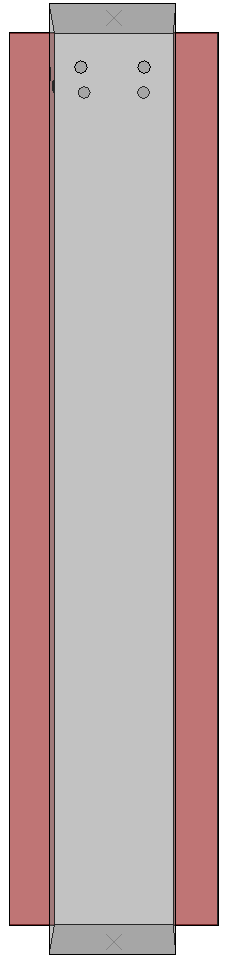
\includegraphics[width=\linewidth]{IMG_CUTRES/a0}
	\end{minipage}
	\quad
	\begin{minipage}[b]{.06\linewidth}
		\centering
		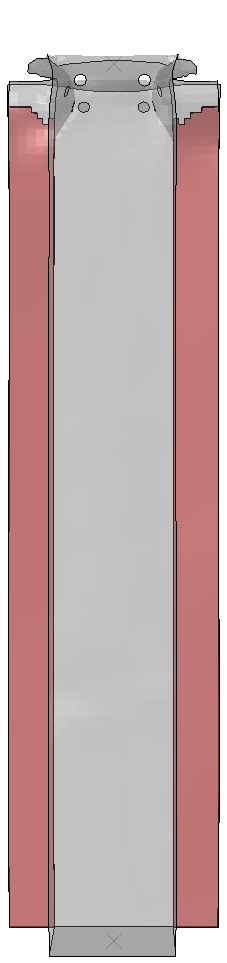
\includegraphics[width=\linewidth]{IMG_CUTRES/a1}
	\end{minipage}
	\quad
	\begin{minipage}[b]{.06\linewidth}
		\centering
		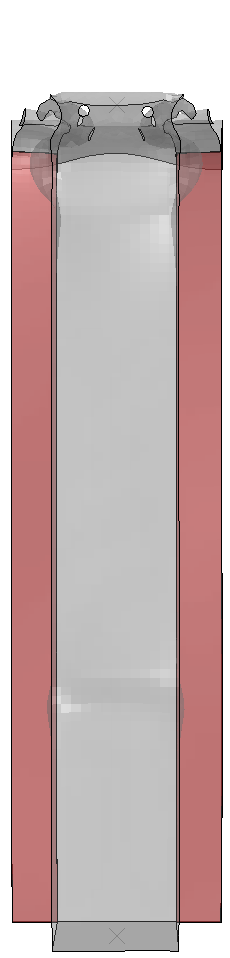
\includegraphics[width=\linewidth]{IMG_CUTRES/a2}
	\end{minipage}
	\quad
	\begin{minipage}[b]{.06\linewidth}
		\centering
		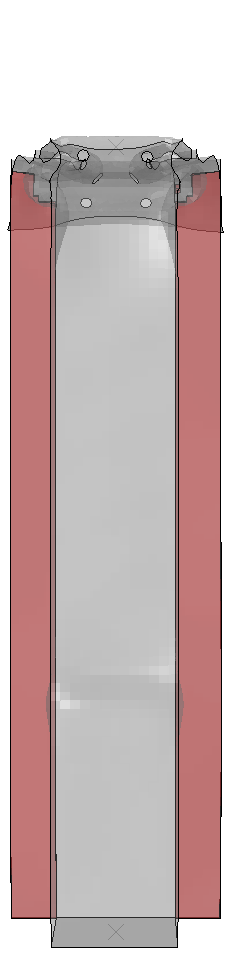
\includegraphics[width=\linewidth]{IMG_CUTRES/a3}
	\end{minipage}
	\quad
	\begin{minipage}[b]{.06\linewidth}
		\centering
		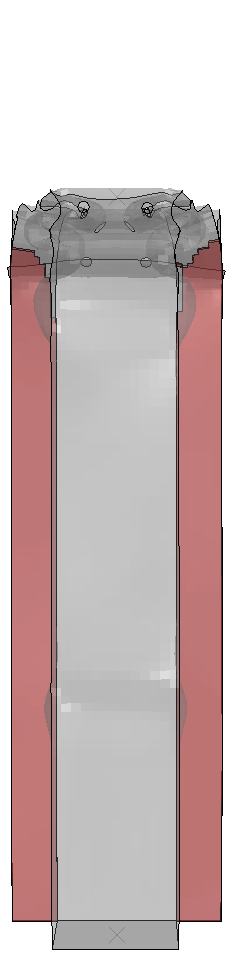
\includegraphics[width=\linewidth]{IMG_CUTRES/a4}
	\end{minipage}
	\quad
	\begin{minipage}[b]{.06\linewidth}
		\centering
		\includegraphics[width=\linewidth]{IMG_CUTRES/a5}
	\end{minipage}
	\quad
	\begin{minipage}[b]{.06\linewidth}
		\centering
		\includegraphics[width=\linewidth]{IMG_CUTRES/a6}
	\end{minipage}
	\quad
	\begin{minipage}[b]{.06\linewidth}
		\centering
		\includegraphics[width=\linewidth]{IMG_CUTRES/a7}
	\end{minipage}
	\quad
	\begin{minipage}[b]{.06\linewidth}
		\centering
		\includegraphics[width=\linewidth]{IMG_CUTRES/a8}
	\end{minipage}
	\quad
	\begin{minipage}[b]{.06\linewidth}
		\centering
		\includegraphics[width=\linewidth]{IMG_CUTRES/a9}
	\end{minipage}
	\quad
	\begin{minipage}[b]{.06\linewidth}
		\centering
		\includegraphics[width=\linewidth]{IMG_CUTRES/a10}
	\end{minipage}

	\caption[Stable collapse mechanism achieved in the top-hat tube with stabilizing box.]{Stable collapse mechanism achieved in the top-hat tube with stabilizing box. Semi-transparent projection with adhesive in red. Total time: $\SI{15}{\ms}$; uniform spacing.}
	\label{fig:stable}
\end{figure}

\begin{figure}
	\centering
	\includegraphics[width=.7\linewidth]{IMG_CUTRES/parallel_stable}
	\caption{Final state on parallel projection with the stabilizing box represented.}
	\label{fig:stabil_box}
\end{figure}

Reaction force is analyzed in this case in order to check the importance share of the stabilizing box on achieving this result. Its F-D is displayed in \cref{fig:stabil_F}, with an equivalent SEA of $\SI{0.30}{\kJ/\kg}$ and peaks of up to $\SI{4.4}{\kN}$. This force has one only component, parallel to the Y axis, which is reminded to be normal to the crushing direction and to the bonding flanges.

\begin{figure}
	\centering
	\includegraphics[width=.7\linewidth]{IMG_CUTRES/RF2_stable}
	\caption{Reaction force on the stabilizing box.}
	\label{fig:stabil_F}
\end{figure}

According to the results displayed on \cref{fig:stable,fig:stabil_box,fig:stabil_F}, it can be concluded that the stabilizing box helps on providing an stable collapse mechanism to the crash tube through the inclusion of a certain force with a minimum SEA input to the system.

\subsection{Factors on absorption of energy}
\label{sec:Ea_factors}

Facing the F-D and different collapse states at several time intervals, an analysis on the relative importance of each factor on Ea is carried out.

The in-plane compression of the rear un-collapsed part of the tube, together with plastic deformation of the frontal end, are the main actors on the base reaction force ---a minimum maintained level that keeps its value almost constant and leaving the variable part to other factors.

Bending waves \textit{per se} do not have great influence on the peaks and valleys series of the F-D, but the adhesive failure pattern does, and it is determined by the former. This means that it is not the adherend plastic deformation the main factor of this variable part, although it has certain variability. \Cref{fig:ads_collapse_progresion} is the case in which this phenomenon can be most easily perceived, as in certain moment, adhesive rapidly fails with very little adherend deformation, and highly increasing the reaction force.

In that same figure, the peak between $\SI{8.25}{\ms}$ and $\SI{10.2}{\ms}$ corresponds to some adhesive final failure (depicted by element removal in the first and second states). The same applies more drastically between the third and fourth states, depicting $\SI{13.2}{\ms}$ and $\SI{15.0}{\ms}$ respectively.

This analysis can be carried out for any other case, with the same conclusions, although this one is the most graphical and the easiest one to be percerived.

\begin{figure}
	\centering
	\begin{minipage}[b]{.35\linewidth}
		\centering
		\begin{minipage}[b]{\linewidth}
		\includegraphics[width=\linewidth]{IMG_CUTRES/AR_RSB_8-25}
		\end{minipage}
		\quad
		\begin{minipage}[b]{\linewidth}
		\includegraphics[width=\linewidth]{IMG_CUTRES/AR_RSb_10-2}
		\end{minipage}
		\quad
		\begin{minipage}[b]{\linewidth}
		\includegraphics[width=\linewidth]{IMG_CUTRES/AR_RSb_13-2}
		\end{minipage}
		\quad
		\begin{minipage}[b]{\linewidth}
		\includegraphics[width=\linewidth]{IMG_CUTRES/AR_RSb_15}
		\end{minipage}
	\end{minipage}
	\quad
	\begin{minipage}[b]{.6\linewidth}
		\includegraphics[width=\linewidth]{IMG_CUTRES/AR_RSb}
	\end{minipage}
\caption[Adhesive collapse influence on F-D.]{Adhesive collapse influence on F-D. Collapse states with semi-transparent adherends and adhesive in red at $\SI{8.25}{\ms}$, $\SI{10.2}{\ms}$, $\SI{13.2}{\ms}$, and $\SI{15.0}{\ms}$; and corresponding F-D. In this case, collapse is started by a mid-point.}
\label{fig:ads_collapse_progresion}
\end{figure}

The possible critical situations that can be developed as a collapse mechanism have varying importance on the final results, strongly depending on the cross section. As commented on \cref{sec:critical_sits}, top-hat section presents minor SEA losses and is more resistant to developing this missfunctions, unlike double hat section.

As of this, it can be concluded that there are three main factors influencing on the value of Ea, being these, in order of importance:
\begin{itemize}
	\item Adherend properties: more specifically its geometry and material.
	\item Adhesive characteristics: specially those involved in its failure, like the fracture energy.
	\item Missfunctional behaviour: although in some cases may be negligible, in others it can be determining.
\end{itemize}

Finally, \cref{tab:sea} summarizes the different obtained SEA values. From there, it can be seen how the top-hat section is not affected in the same magnitude in the final SEA value as the double hat section, although the collapse mechanism may change by transferring the wave formation process to other part of the tube and certain other corresponding implications. The obtained values are close to those experimentally obtained by \cite{Peroni2009}, giving certain credit on the goodness of the results of the present study.

On the other hand, the double hat section SEA obtained values drastically change when modifying the contact interaction properties, dropping to between $82\%$ and $63\%$ of values with other interaction definition, and about a half or even a third of the experimental values obtained by \cite{Peroni2009}. The rough case with stabilization box seems to get the closest to resembling cited experiments, although its collapse mechanism is not the same, as the modeled one generates waves in the mid-tube, as can be seen on \cref{fig:best_B_tube}

\begin{figure}
	\centering
	\includegraphics[width=0.7\linewidth]{IMG_CUTRES/best_B_tube}
	\caption[Collapse of the double hat section tube with stabilization box and rough contact property.]{Collapse of the double hat section tube with stabilization box and rough contact property. Adhesive in blue. SEA: $\SI{7.34}{\kJ/\kg}$.}
	\label{fig:best_B_tube}
\end{figure}


% \begin{table}[htpb]
% 	\centering
% 	\begin{tabular}{llcc}
% 		\hline
% 		\multirow{2}{*}{Contact} & \multirow{2}{*}{Situation} & \multicolumn{2}{c}{Cross section} \\ \cmidrule{3-4}
% 		\multicolumn{2}{l}{}                                    & Top-hat         & Double hat     \\ \hline
% 		\multirow{4}{*}{Rough}                  & -             & $5.43$          & $5.20$         \\
% 		& R             & $5.36$          & $6.08$          \\
% 		& Sb            & $5.70$          & $7.34$          \\
% 		& RSb           & $5.61$          & $6.69$          \\ \hline
% 		\multirow{4}{*}{Frictionless}           & -             & $4.21$          & $3.32$         \\
% 		& R             & $5.50$          & $3.86$         \\
% 		& Sb            & $5.55$          & $5.88$          \\
% 		& RSb           & $5.40$          & $5.51$          \\ \hline
% 	\end{tabular}
% 	\caption[SEA summary.]{SEA summary. ``R'' stands for riveted tube; ``Sb'', for tube with stabilizing box; ``RSb'', for both simultaneously.}
% 	\label{tab:sea}
% \end{table}

\subsection{On load standard deviation}

Facing the factors that were concluded on \cref{sec:Ea_factors}, the SD value of the F-D can be interpreted also as a measure of the progressiveness or the suddenness of the failure of the crash box, specially and more specifically of the adhesive.

% \begin{table}[htpb]
% 	\centering
% 	\begin{tabular}{llcc}
% 		\hline
% 		\multirow{2}{*}{Contact} & \multirow{2}{*}{Situation} & \multicolumn{2}{c}{Cross section} \\ \cmidrule{3-4}
% 		\multicolumn{2}{l}{}                                    & Top-hat         & Double hat      \\ \hline
% 		\multirow{4}{*}{Rough}                  & -             & $6.79$          & $10.47$         \\
% 		& R             & $6.60$          & $8.84$          \\
% 		& Sb            & $8.04$          & $6.80$          \\
% 		& RSb           & $7.25$          & $7.73$          \\ \hline
% 		\multirow{4}{*}{Frictionless}           & -             & $5.76$          & $11.91$         \\
% 		& R             & $5.53$          & $10.72$         \\
% 		& Sb            & $5.29$          & $8.65$          \\
% 		& RSb           & $4.97$          & $8.82$          \\ \hline
% 	\end{tabular}
% 	\caption[SD summary.]{SD summary. ``R'' stands for riveted tube; ``Sb'', for tube with stabilizing box; ``RSb'', for both simultaneously.}
% 	\label{tab:standard_dev}
% \end{table}

In general terms, top-hat section shows a better performance in terms of SD, as it can be seen on \cref{tab:standard_dev}, likely thanks to its better resistance to developing critical situations. Both rough cases with stabilizing box on rough contact conditions seem to be the exception to the tendency, as the top-hat tube shows a larger SD than the double hat one. Their F-D is depicted in \cref{fig:R_Sb}. A similar phenomenon happens on those cases that add rivets to these ones, although not in an enough magnitude to make the double hat section value bigger than the top-hat section one.

\begin{figure}
	\centering
	\includegraphics[width=0.7\linewidth]{IMG_CUTRES/R_Sb}
	\caption{F-D of models with rough contact and stabilizing box.}
	\label{fig:R_Sb}
\end{figure}

Although none of these cases depicts a critical situation, they behave differently to other similar tests. Analyzing the collapse mechanism in the top-hat section, the rapid mode II failure at certain stages creates local peaks also explained in \cref{sec:final_tendency} that are related to the variability of the F-D.

Concurring with this situation, on the other hand, the double hat section shows in these cases some of the most stable collapses among the obtained results, allowing thus a more balanced result against its counterpart. In spite of being fairly stable, its SD is still particularly high if compared to many top-hat section results. Analyzing the F-D, the peaks and valleys series is included in a general downwards tendency, unlike other series which oscillate among a fairly constant level. This implies that SD is not the perfect tool for measuring the stability of the collapse mechanism, although it is good enough to give an idea.

Double hat section on frictionless contact conditions, whose F-D are represented in \cref{fig:F-D_frictionless}, present the greatest values of SD among the modeled tubes. In spite of the similarities between these curves, the showed collapse mechanism is different between those with and without stabilizing box, although the causes are fairly the same: a great valley after the Pk followed by a second local peak around $\num{8}\sim\SI{10}{\ms}$.

The cases without stabilizing box find the genesis of this late peak in the developed critical situation, which corresponds to a general bending case. As \cref{fig:gen_bend_weakening} shows, the peak implies the final dispossure of Ea by the frontal part of the tube, as it completely bends over itself. Beyond this point, this frontal part does not intervene any more, and the collapse starts again in some way from this moment only using the capabilities of the rest of the tube.

\begin{figure}
	\centering
	\begin{minipage}[b]{.3\linewidth}
		\centering
		\includegraphics[width=\linewidth]{IMG_CUTRES/b1}
		$\SI{7.5}{\ms}$
	\end{minipage}
	\quad
	\begin{minipage}[b]{.3\linewidth}
		\centering
		\includegraphics[width=\linewidth]{IMG_CUTRES/b2}
		$\SI{8.25}{\ms}$
	\end{minipage}
	\quad
	\begin{minipage}[b]{.3\linewidth}
		\centering
		\includegraphics[width=\linewidth]{IMG_CUTRES/b3}
		$\SI{9.0}{\ms}$
	\end{minipage}
	\caption[Final collapse dispossure of the frontal part of the tube in a general bending case.]{Final collapse dispossure of the frontal part of the tube in a general bending case. Adhesive in blue.}
	\label{fig:gen_bend_weakening}
\end{figure}

In those cases with stabilizing box, this process aims to develop, but it is stopped by the mentioned device, which does not prevent the second peak. Big bending waves are developed within the stabilizing box on its place. After the great valley between $\SI{2}{\ms}$ and $\SI{7}{\ms}$, approximately, force values scale up back again, finding a second peak with similar origin and characteristics as the one mentioned for the previous case. From that point, more energy is absorbed mainly due to adhesive failure. In the final stages, the currently forming wave implodes the cross section. In general terms, this collapse mechanism is fairly chaotic ---as local collapse patterns change from one point to another instead of developing the same in the whole tube---, in spite of being stabilized.

\subsection{Final raising tendency}
\label{sec:final_tendency}
% Explain tendency on the final stages to great values

Several models with stabilizing box and rough contact were found to scale up the transmitted load in the last stages of the impact, thus deviating from the reference values, and reaching values close to the Pk that takes places in the first moments of the impact. F-D of this models are depicted in \cref{fig:AR_Sb}.

\begin{figure}
	\centering
	\includegraphics[width=0.7\linewidth]{IMG_CUTRES/AR_Sb}
	\caption{Top-hat section models with rough contact developing high values of transmitted load in the last stages of the impact.}
	\label{fig:AR_Sb}
\end{figure}

Analyzing the collapse path, this tubes show wave formation in the mid-rear part of the tube. The wave size has relation with the big peak of the middle of the analysis. The frontal part of the box seems to enter an in-plane compression of the adherends in the last phases of the impact, with high shear effort between adherends.

This leads to a rapid energy release due to adhesive mode II failure in the last moments of the analysis, likely creating the last peak of the analysis.

Although the final Ea is relatively similar to other cases, this last peak on loading is considered totally undesirable, as it reaches values of more than $80\%$ of Pk which would increase injury suffered by vehicle passengers.

\subsection{Model deviations}
The present section aims to expose some of the differences found between the developed models and the results of reference given mainly by \cite{Scattina2011} and \cite{Peroni2009}.

Obtained curves present a first peak of $\num{45}\sim\SI{50}{\kN}$ in the beginning of the impact, and then a series of peaks, less pronounced and lower in value, alternating with valleys during the wave formation, with a mean value of $\num{10}\sim\SI{20}{\kN}$. Reference values were found to be alike, being the main exception on the double-hat section, which has lower peak and mean force value.

The main exception to these similitudes can be found on the first peak, specially with rough interaction property, which progressively reduces its value after happening, instead of rapidly dropping its magnitude to the peaks and valleys series' mean. It is believed that this situation may be related to the crushing speed. On a quasi-static experiments and models, test velocity allows stresses to re-accommodate; meanwhile, on impact tests, this redistribution can be appreciated thanks to the scale of time.

\subsection{Critical situations results}

\Cref{tab:critical_sits} summaries the SEA values obtained in the present study for the different critical situations that were experienced. As shown, top-hat section crash boxes decay less when happening, being thus much more reliable solution for this use.

\begin{table}
	\centering
	\begin{tabular}{lcc}
		\hline
		Critical situation 						& Top-hat 		& Double hat 	\\
		\hline
		None 									& $\num{5.55}$	& $\num{7.34}$ 	\\
		Triggering misfunction 					& $\num{4.21}$	& $\num{5.13}$ 	\\
		General bending 						& Unfound		& $\num{4.79}$ 	\\
		General peeling due to plates buckling 	& Unfound		& $\num{4.28}$ 	\\
		\hline
	\end{tabular}
	\caption[Summary of SEA values on different critical situations.]{Summary of SEA [$\si{\kJ/\kg}$] values on different critical situations. Mean values given in case of being found several times. \cite{Peroni2009} obtained $\SI{4.8}{\kJ/\kg}$ and $\SI{10.3}{\kJ/\kg}$ respectively for top-hat and double hat sections.}
	\label{tab:critical_sits}
\end{table}

It is also very remarkable the significantly high values of SD in this situations, motivated by the strong variabilities in their corresponding force-displacement curves (see \cref{fig:tmf_fd,fig:gppb_fd}).

In case of triggering missfunction, it reaches $\SI{11.66}{\kJ/\kg}$, a value alike the most unfavorable found in this study. The general peeling due to plates buckling case is $\SI{32.99}{\kJ/\kg}$. It should be remarked that, because of the definition of this parameter, this value is not as high as it may look like, as the mean values of these both force-displacement curves is $\SI{14.78}{\kJ/\kg}$ and $\SI{28.76}{\kJ/\kg}$, respectively.

\todo{Poner bien las referencias (citet pero que funcione)}
\section{Optimization strategy}




\subsection{Surrogate-based methods}

In order to optimize the specimen, a surrogate-optimization approach is used. Therefore, the computationally-expensive  objective functions of the model are replaced by another functions less costly to evaluate. 

Firstly, with the parametrized model, a sampling of !!N!!\todo{!!} samples is performed, relying on the LHS technique. This method creates a set of data with homogeneous projections on each variable axis, so that no superimposed projections appear. 

Once the sampling is obtained, the surrogate model is created. The Multivariate adaptive regression splines (MARS) method is chosen, where the surrogate functions are adjusted with cubic splines following the next expression
\begin{equation}\label{eq:mars}
\hat{f}\left ( \bm{x} \right )= \sum_{m=1}^{M}a_{m}B_{m}\left ( \bm{x} \right ),
\end{equation}
where $B_{m}$ are the power basis functions, $a_{m}$ the coefficients of the functions, and $M$ is the number of functions. This method is more thoroughly explained in \cite{Friedman1995197}. 

In order to judge the accuracy of the trend functions, the goodness of fit $R^2$, needs to be looked into. This indicator is defined as
\begin{equation}\label{eq:correlation_coefficient}
  R^2 = {\left(\dfrac{\sigma_{\bm{f}
\bm{\hat{f}}}}{\sqrt{\sigma_{\bm{f}}^2
\sigma_{\bm{\hat{f}}}^2}}\right)}^2
\end{equation}

This is done for all objective functions, where values equal or higher than $0.95$ for the selected objective functions are expected. 

With the surrogate-based model created, two optimization strategies are used. In a first approach, single-objective optimization techniques are applied. The calculations that this type of optimization requires are relatively simple once the proper surrogate model has been built. Single-objective optimization searches for the minima of the function within the limits of the design space. Traditional methods involving gradient-based and Hessian-based information are not very useful for optimizing the type of problems studied in this research, since many local minima are found in the function, yielding only misleading results. Therefore, a single-objective evolutionary algorithm is used, since this type of methods are slower but dodge local minima with ease.

The other type of optimization used is multi-objective optimization. This procedure involves more resources for the calculations. Instead of a single point, the results are conformed by a Pareto front, corresponding to a range of results. The set of all Pareto optimal design configurations, $P^*$, is defined as:

\begin{equation}
P^* := \left\{ x \in \Pi \   \nexists x' \in \Pi \    \hat{f}_i \left( \bm{x'} \right) \leqslant \hat{f}_i \left( \bm{x} \right)  \right\}
\end{equation}
and the Pareto front, which is the set of optimal objective functions from the Pareto design configurations, $PF^*$, is defined as:

\begin{equation}
PF^* := \left\{ \overline{\bm{u}} = \left( \hat{f}_1 \left( \bm{x} \right), \ldots , \hat{f}_k \left( \bm{x} \right) \right)  x \in P^* \right\}
\end{equation}

In the end, the set of points from the Pareto front has a number of components equal to the number of objective functions, each constituting a feasible solution to the problem. This Pareto front points cannot improve the value of one objective function without worsening the value of at least one other objective function. \Cref{fig:Pareto} shows an example of a Pareto front opposing the energy absorbed by the specimen and its mass, where the line constitutes the set of optima for these metrics.

\begin{figure}[htpb]
  \centering
   \includegraphics[width=.8\columnwidth]{figures/IMG/Pareto}
  \caption{Pareto frontier opposing energy absorbed and mass of the specimen.}
  \label{fig:Pareto}
\end{figure}

Therefore, the results shall be analyzed and, depending on the needs required for the specimen, one or other point on the frontier is chosen. As with the single-objective optimization, multi-objective optimization usually has problems with local minima. For this problem, genetic algorithms are used, aiming for better and more reliable results.

The methods selected for both the single- and the multi-objective optimization are the genetic algorithms from the JEGA Library, developed by \cite{JEGA}. This methods perform optimization supporting general constraints as well as mixtures of real and discrete variables. The variables are encoded and referred to as chromosomes, and each digit of the variable is a gene.

\subsection{Metrics}
\todo{Plagiado}
The objective of this research is to find a set of optimum designs of the specimen previously described according to three different objective functions. These functions are the absorbed energy ($E_a$), the mass of the specimen ($m$) and the peak load ($P_{peak}$). The three metrics are obtained using a finite element simulation, where $E_a$ and $P_{peak}$ are obtained via the force-displacement curves.

Before making any calculations with the force-displacement curve, and according to the specialized literature in crash analysis \cite{Huanglibro}, a standard SAE 600 filter \cite{J211} is applied. This removes the high-frequency noise from the curve with a cutoff frequency of ${1000}$ Hz. Once the filter is used, the direct integration of the resulting force-displacement curve yields to the $E_a$:
\begin{equation}\label{Ea}
  E_{a}=\int _{0}^{\delta }F\! \left( z \right) \,dz\,,
\end{equation}
with $\delta$ being the total axial crushing distance and $F\! \left( z \right)$ the value of the crushing force at the crushing length $z$.

The peak load $P_{peak}$ is defined as
\begin{equation}\label{Peak}
 P_{peak}=max\left\{ F\! \left( z \right)  \forall z \in [0,\delta] \right\}
\end{equation}

These three objective functions have not been randomly chosen. The first reason is the nature of the design and its aim to improve the crashworthiness of vehicles. The $E_a$ can be easily improved by increasing the thicknesses of the materials, but this would harm the other two objective functions $m$ and $P_{peak}$, increasing both of them. An increase in the mass of the specimen translates into a higher mass of the vehicle, increasing its fuel consumption and reducing its performance; whereas an increase in the $P_{peak}$ means a higher force and acceleration suffered by the passengers of the vehicle, raising the odds of resulting in a serious injury.

The second reason for choosing these objective functions is purely computational. Traditionally, other researchers have swerved towards optimization of the specific energy absorption (SEA) and the load ratio (LR) \cite{Hou2007555}. The SEA function is defined as a ratio between $E_a$ and $m$:
\begin{equation}\label{SEA}
  S\! EA=\dfrac {E_a} {m}
\end{equation}

By contrast, the load ratio relates the $P_{peak}$ with the mean load $P_m$ as
\begin{equation}\label{LR}
  LR=\dfrac {P_{peak}} {P_m}
\end{equation}

The mean load is obtained as a ratio between the absorbed energy and the total crushing length $\delta$:
\begin{equation}\label{Pm}
  P_{m}=\dfrac {E_a} {\delta}
\end{equation}

The SEA and LR were also evaluated as objective functions, but it was found that during the optimization process these quantities have a more complicated comportment and a noisier nature for this model. Consequently, they were only used during the parameter study and the single-objective optimization. They were discarded from the multi-objective  optimization process and are only used as indicators to compare different specimens.

The peak load is also used as a constraint in the single-objective optimization. This is done so that, in the real specimen, the required force to crumple the piece is never over a certain value, thus protecting the rest of the car's chassis and the occupants. In the multi-objective optimization this is not required nor used, since the final results consist of Pareto fronts, where the maximum peak load depends on the mass or energy absorption desired.

\subsection{Optimization process}

In order to optimize the model, the process has been divided into different stages. Firstly, a parameter study is performed. A simple sampling of the work space for each variable is carried out. With this, a general idea of the variables' behavior is obtained.

Secondly, single-objective optimization is run for the SEA objective function. Whereas an optimization of the mass and the absorbed energy would provide better results, this can be easier optimized, since the other option requires multi-objective optimization. Both unconstrained and constrained optimization procedures are considered, setting a limit for the peak load constraint in the latter.

Lastly, multi-objective unconstrained optimization is sought. All objective functions are minimized, and the points obtained as solution cannot be improved in a variable without harming, at least, another one. This last step is the most complete, giving more information of the behavior of the functions and the optimization process, but due to the greater complexity in the evaluation it is computed the last.

Starting from a baseline model, the optima greatly improve the performance of the model. \Cref{fig:opt_comparison} shows the section of both a baseline model and the single-objective optimum for a maximized SEA. \todo{Te falta el caption. El label ya se lo puse yo.}

\begin{figure}[htpb]
\begin{subfigure}[b]{.45\columnwidth}
   \includegraphics[width=\columnwidth]{figures/IMG/sc1.pdf}
    \caption{Baseline model.}
    \label{fig:back0}
\end{subfigure}
\qquad
\begin{subfigure}[b]{.45\columnwidth}
   \includegraphics[width=\columnwidth]{figures/IMG/topview.png}
    \caption{Specimen with optimum SEA.}
    \label{fig:back5}
\end{subfigure}
\caption{blablabla}
\label{fig:opt_comparison}
\end{figure}


\section{Conclusions}
\todo{Quitar el usepackage todonotes}
\section{Acknowledgments}



\bibliography{./references/references}

\end{document}
